\section{Introduction}
This section will talk about all the design choices made in the creation of my Robotron inspired remake. This primarily includes a hierarchy chart, consisting of my objectives. However, it is important to note that this is more of a structure of how each objective interacts. The system interacts through MVC, and as such, i will also focus heavily (but in a different section) into the way in which MVC actually works, on a lower level, using pseudo code and diagrams to explain the entire system workings. This has been separated out of the hierarchy charts to avoid confusion.

\section{Hierarchy Charts}
The first chart sets the layout for the others. The chart had to be divided into smaller sections to allow for readability and easier implementation guidance. 

\begin{figure}[H]
  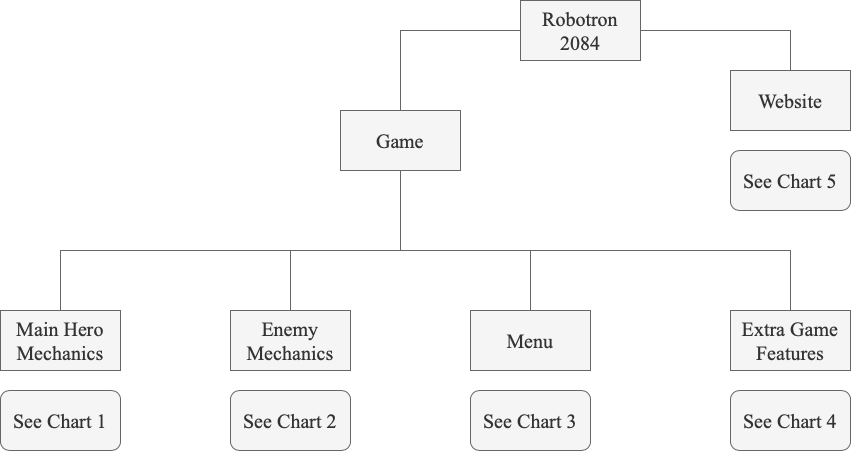
\includegraphics[width=0.8\linewidth]{Figures/chart0.png}
  \centering
  \caption{The first chart showing the basic overview}
  \label{fig:Chart_0}
\end{figure}

\begin{figure}[H]
  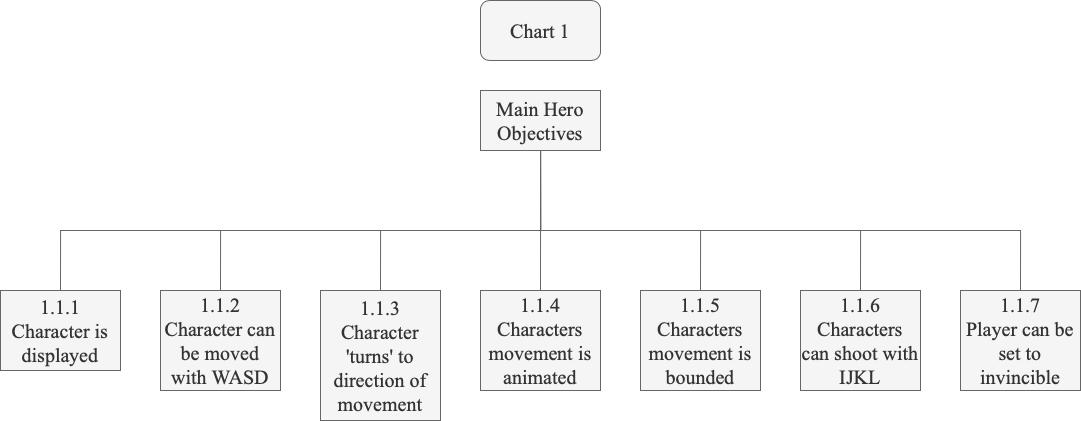
\includegraphics[width=1\linewidth]{Figures/chart1.png}
  \centering
  \caption{Chart detailing Main Hero Mechanics}
  \label{fig:Chart_1}
\end{figure}

\begin{figure}[H]
  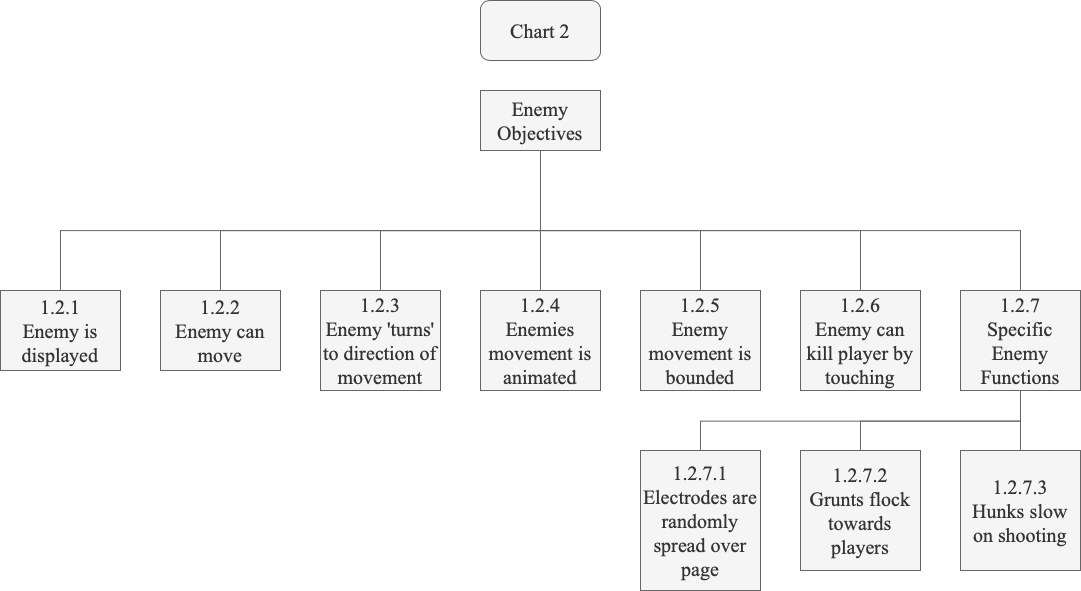
\includegraphics[width=1\linewidth]{Figures/chart2.png}
  \centering
  \caption{Chart detailing Enemy Mechanics}
  \label{fig:Chart_2}
\end{figure}

\begin{figure}[H]
  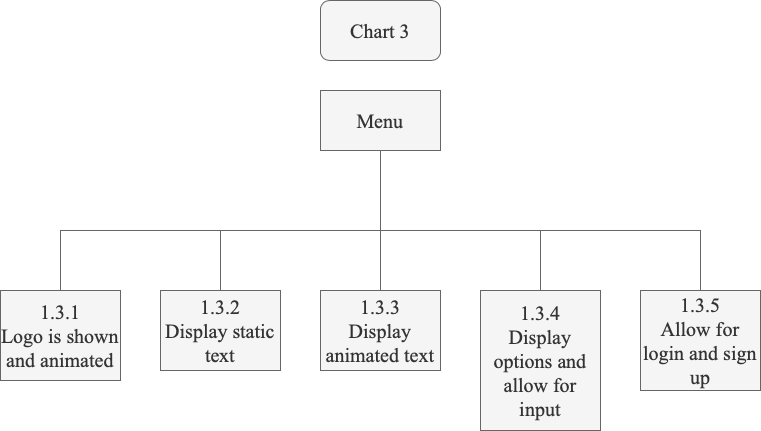
\includegraphics[width=0.6\linewidth]{Figures/chart3.png}
  \centering
  \caption{Chart detailing menu}
  \label{fig:Chart_3}
\end{figure}

\begin{figure}[H]
  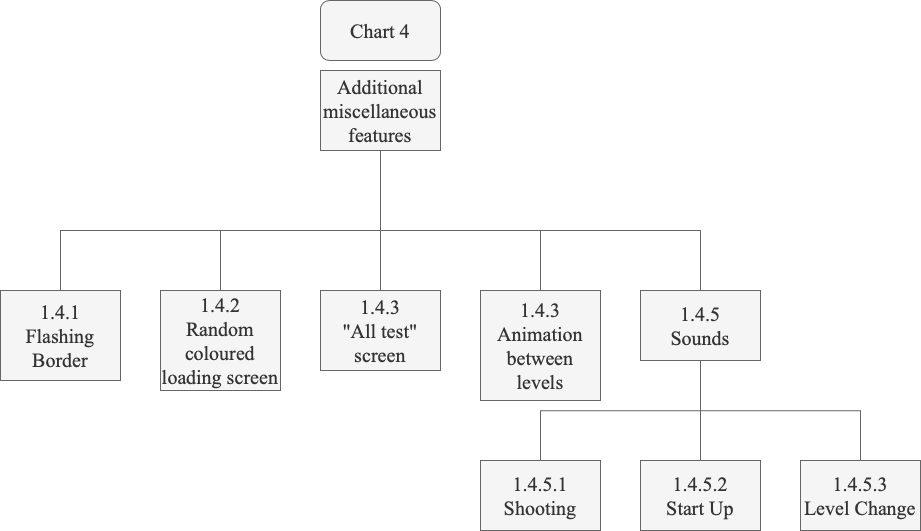
\includegraphics[width=1\linewidth]{Figures/chart4.png}
  \centering
  \caption{Chart detailing miscellaneous features}
  \label{fig:Chart_4}
  
\end{figure}
\begin{figure}[H]
  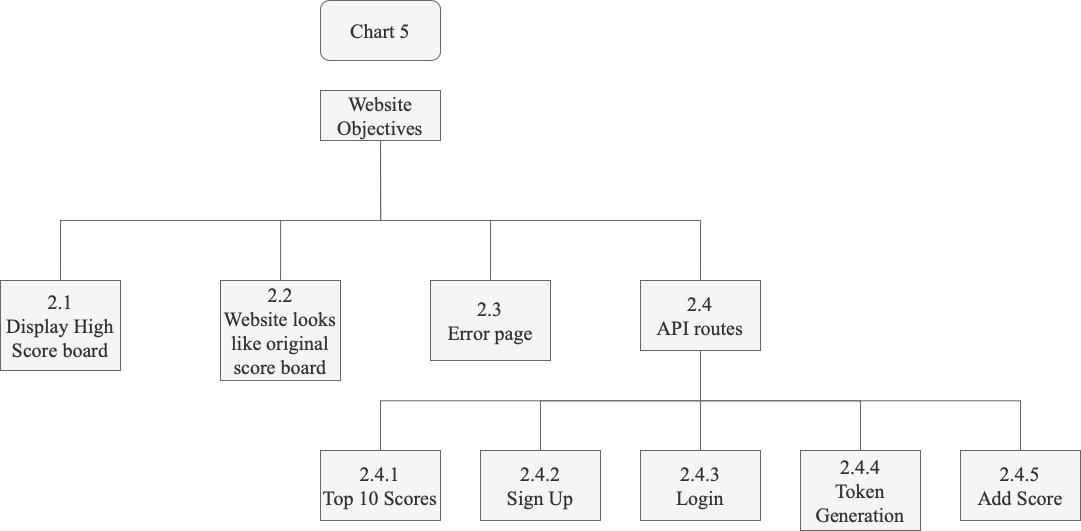
\includegraphics[width=1\linewidth]{Figures/chart5.png}
  \centering
  \caption{Chart detailing website features}
  \label{fig:Chart_5}
\end{figure}

\section{Class Diagrams}
These diagrams define what the actual implementation of classes will be, the first diagram shows that there is a lot of emphasis here on the inheritance and relationships between the classes, its worth noting some of these may extend from default pygame classes, like a surface or sprite, the diagram does show all the classes I have implemented though - along with all of their functions and attributes. 
\begin{figure}[H]
  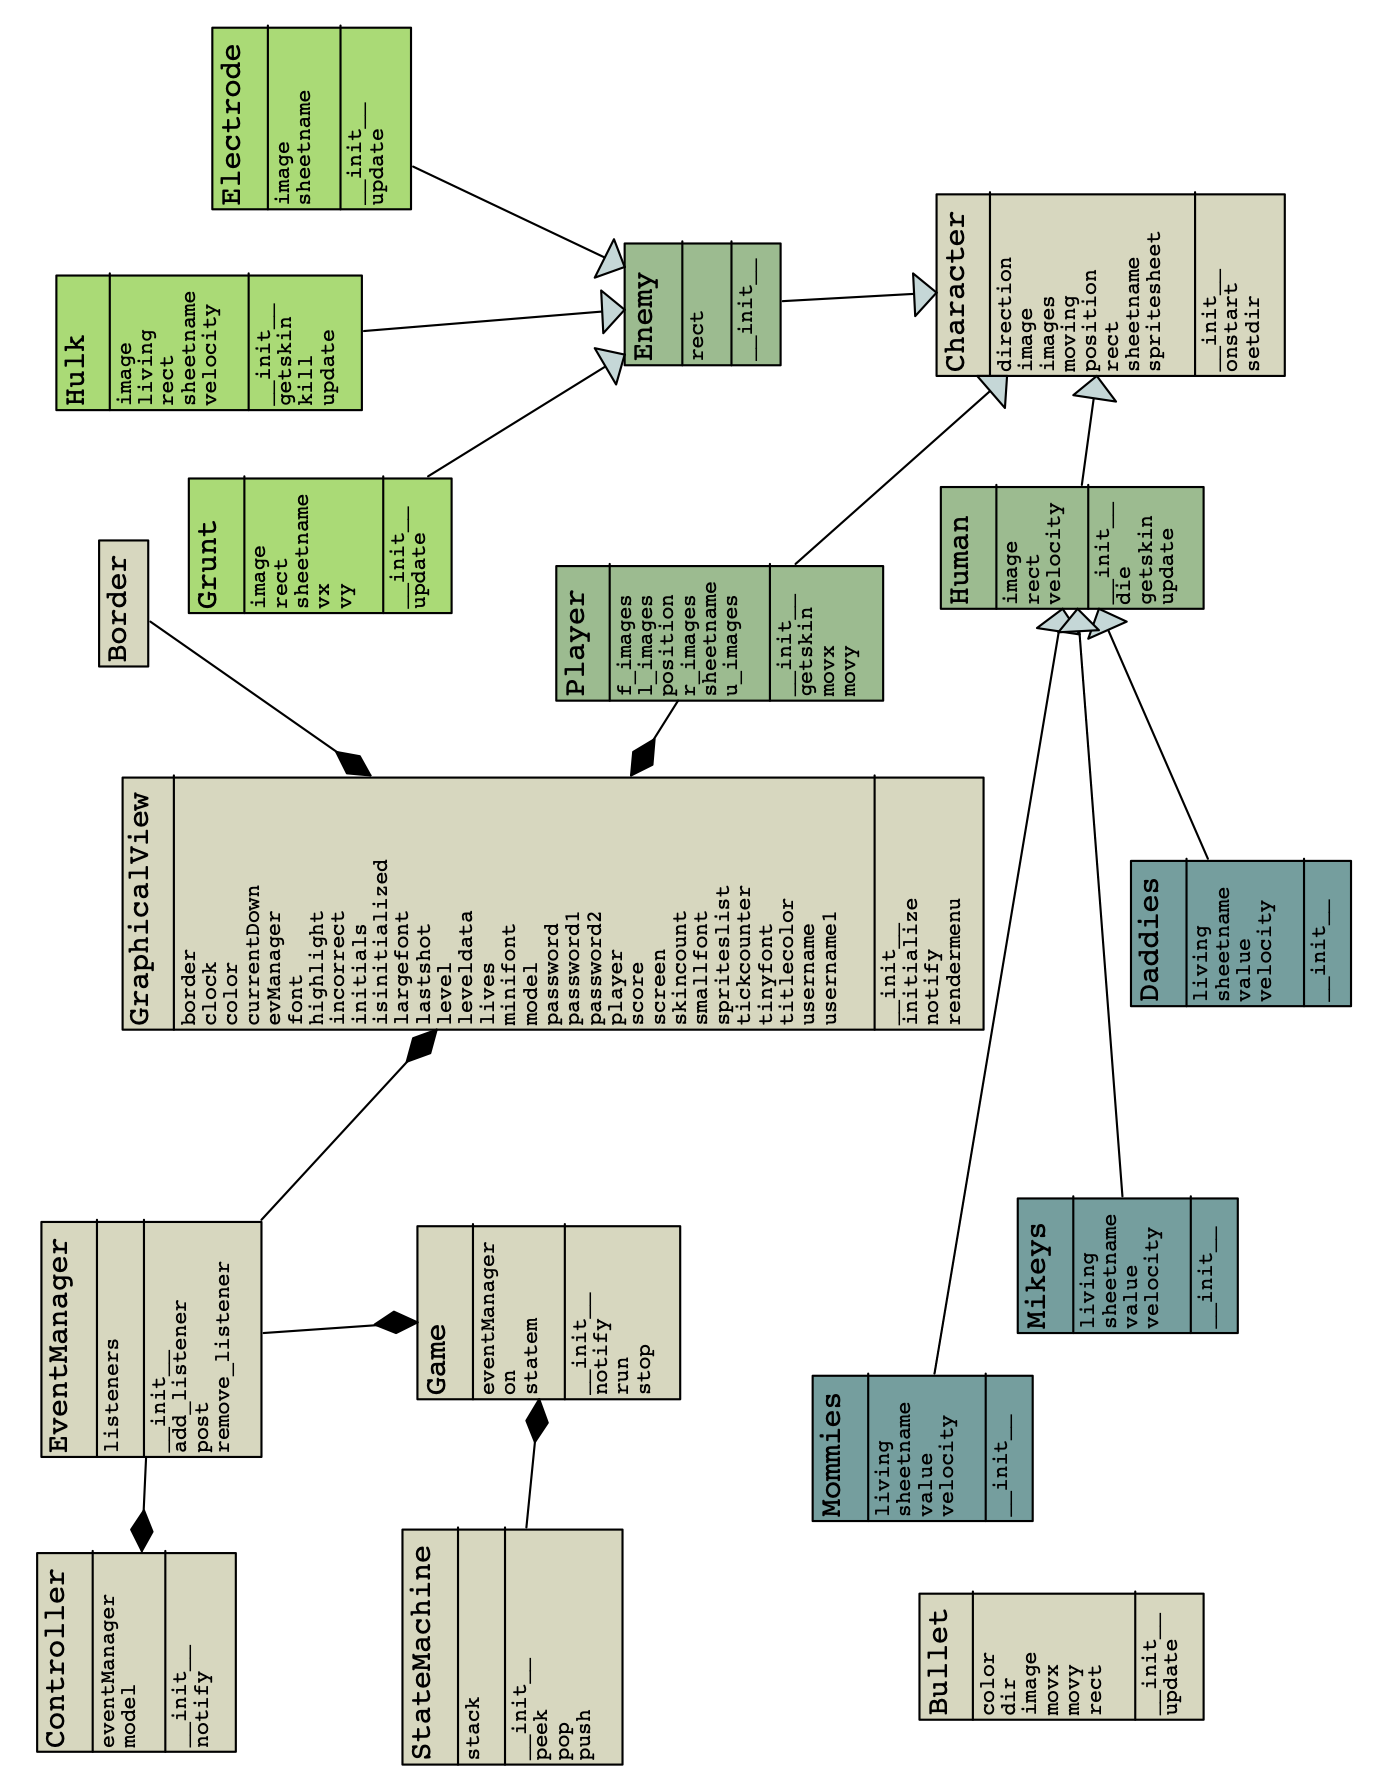
\includegraphics[width=1\linewidth]{Figures/overallclassdiagram.png}
  \centering
  \caption{Class diagrams for the entire system}
  \label{fig:Class_Diagram_MAIN}
\end{figure}

\begin{figure}[H]
  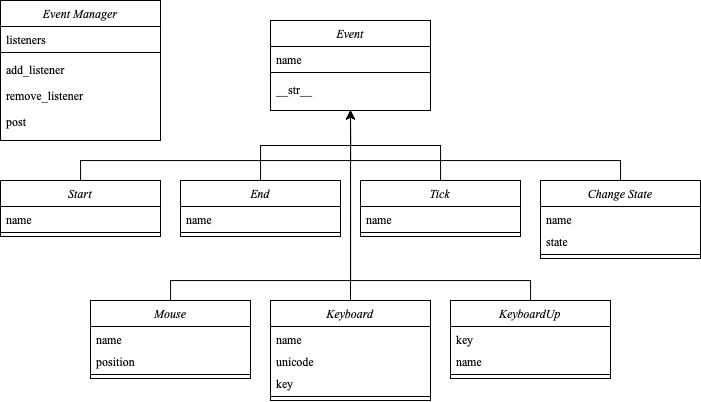
\includegraphics[width=1\linewidth]{Figures/eventclass.png}
  \centering
  \caption{Class diagrams for the events and event manager}
  \label{fig:Class_Diagram_1}
\end{figure}

\begin{figure}[H]
  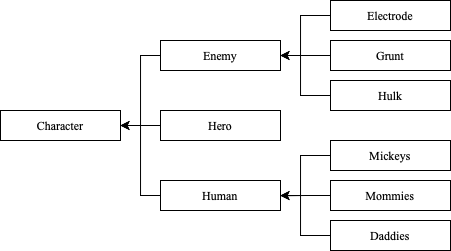
\includegraphics[width=0.6\linewidth]{Figures/charactersDiagram.png}
  \centering
  \caption{Class diagram (with methods and attributes hidden) for characters}
  \label{fig:Class_Diagram_2}
\end{figure}

\begin{figure}[H]
  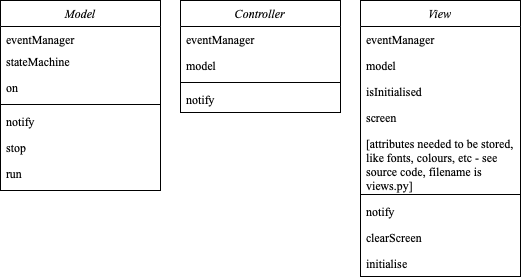
\includegraphics[width=0.8\linewidth]{Figures/MVC0.png}
  \centering
  \caption{Classes required for MVC}
  \label{fig:Class_Diagram_3}
\end{figure}

\section{Key Algorithms}
\subsection{Boids Flocking}
Whilst the maths for this was covered in the  analysis, I will here run through with some pseudo code to show how the moves will be calculated. This pseudo code will be run every time there is a tick emitted (such that the positions are updated every tick - more on ticks in the next section).

\begin{lstlisting}
SUB boids(grunt, gruntlist, playerpos)
    
    # Initialise the variables
    
    x_total, y_total = 0,0
    centre_x ,centre_y = 0,0
    velocity_x, velocity_y = 0,0
    
    # We need this to find all the averages for velocity and positions
    count = len(gruntlist)
    
    # Loop through the grunts on screen
    FOR var_grunt IN gruntlist:

        # Add their positions to the total counts
        x_total += var_grunt.x
        y_total += var_grunt.y
        
        # If they are within 60 pixels of the current grunt - some Pythagoras here
        IF SQRT((var_grunt.x-grunt.x)**2 + (var_grunt.y-grunt.y)**2) < 60 THEN
            # This is the implementation for rule 2 - avoids collisions
            centre_x += centre_x - (var_grunt.x-grunt.x)
            centre_y += centre_y - (var_grunt.y-grunt.y)
            centre_x += (playerpos.x - grunt.x) / 2
            centre_y += (playerpos.y - grunt.y) / 2
        ENDIF
        
        # Add their velocities to the total counts
        velocity_x += var_grunt.velocity_x
        velocity_y += var_grunt.velocity_y
    
    ENDFOR
    
    # Move the grunt closer to the player
    p1 = (playerpos.x-grunt.x) /5
    p2 = (playerpos.y-grunt.y) /5

    # Work out all the averages
    xavg, yavg = x_total/count, y_total/count
    vxavg, vyavg = velocity_x/count, velocity_y/count
    
    # Return (after weighting the rules)
    RETURN (xavg/100)+c1+(vxavg/20)+p1, (yavg/100)+c2+(vyavg/20)+p2
ENDSUB
\end{lstlisting}

\subsection{MVC}
MVC plays a big part in this system and how it works. This is backed by an event and state system too. The class diagrams gave a high level overview of how this works, but no detail into how they interact. This is what will be explained in this section.

Everything is, in reality, centred around the events. These are all controlled by the event manager. The event manager emits messages (or events) to the model, view and controller. These are all received through the 'notify' method on the classes (as each class has this function, the for loop can call the method on all the 'listeners'). The function then decides what it needs to do. Some events may be entirely ignored by the class, whilst others are needed. As such, each event type is its own subclass of the general event. An example of this is the model, which only really relies on the change state and end game events, whilst the view uses all of them.

The states are also needed, the view uses these most of all. The states help it know what generally belongs on screen, whilst the tick counter is what can fine tune that when needed (only certain screens need this, like the menu). So, this flowchart will run through what a basic game might look through.
\begin{figure}[H]
  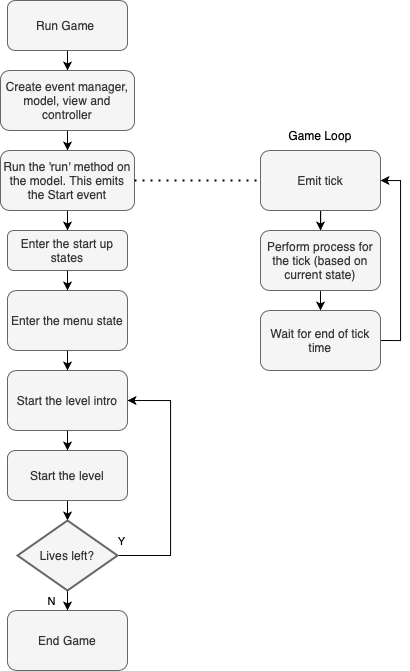
\includegraphics[width=0.7\linewidth]{Figures/flowchart.png}
  \centering
  \caption{Flowchart of how data flows through the system}
  \label{fig:flowchart}
\end{figure}

\subsection{Security}
The project needs security in a few spots. For example, it uses bcrypt, a key derivation algorithm to store passwords. This is much more effective than simply just hashing. It hashes the password, along with salting it, to make it invulnerable to rainbow tables. It then repeats, over and over. This means it takes time to calculate. The idea of a key derivation algorithm over a simple hashing algorithm like SHA is to make computing the result difficult. 

Another aspect where security will be important is in the token generation. If it were possible to guess the token, then a user could authenticate as a different user. As such, I use secrets, specifically the token\_urlsafe, to generate a cryptographically secure, 30 character token. 

\section{Storing Data}
This project stores data in 2 ways. First, some data is stored in levels.csv, but this is hard coded and not changed through the games running. .tokens is a file (hidden to users with the file name starting with a .) which stores the token. It isnt an issue for this to be stored plain text, so it stored in the file, along with the user name, separated with a > between them.
\section{Data Structures}

\subsection{Stack}
A stack is a LIFO (last in, first out) data structure. It quite literally acts as a stack of objects. This is what the state machine uses to transition between and store states. This is implemented with a list, objects are both added to and removed from the end, so this is rather simple, but i have included the pseudocode below. 

\begin{lstlisting}
CLASS StateMachine
    stack = []
    
    SUB peek
        TRY
            RETURN stack[-1]
        EXCEPT
            RETURN None
        ENDTRY
    ENDSUB
    
    SUB pop
        TRY
            stack = stack[1:]
            RETURN LEN(stack)
        EXCEPT
            RETURN None
        ENDTRY
    ENDSUB
    
    SUB push(state)
        stack.append(state)
        RETURN state
    ENDSUB
ENDCLASS
\end{lstlisting}
\section{API and Website Design}
The table below shows the routes available on the API, as explained in analysis, this API is used to return the top 10 users, login in, sign up, and validate tokens - forming most of the admin tasks, as well as the website. The website uses a template in flask to show a screen like the original high screen board. The images below show the original and my replica of the high score board. [source for original image \url{http://highscore.com/scores/GameCube/MidwayArcadeTreasures/58417}]

\begin{table}[!ht]
\begin{tabular}{|l|l|l|}
\hline
\rowcolor[HTML]{C0C0C0} 
ROUTE            & METHOD & DESCRIPTION                                                  \\ \hline
/leaderboard     & GET    & Returns JSON of top 10 users (initials + scores) in Database \\ \hline
/user/userid     & GET    & Returns JSON of top score                                    \\ \hline
/username/userid & GET    & Returns ID of given username                                 \\ \hline
/login           & POST   & Logs in a user, sends token, or logs user in with token      \\ \hline
/addscore        & POST   & Adds a score, given score and a token                        \\ \hline
/adduser         & POST   & Adds a user to the database                                  \\ \hline
\end{tabular}
\end{table}


\begin{figure}[H]
  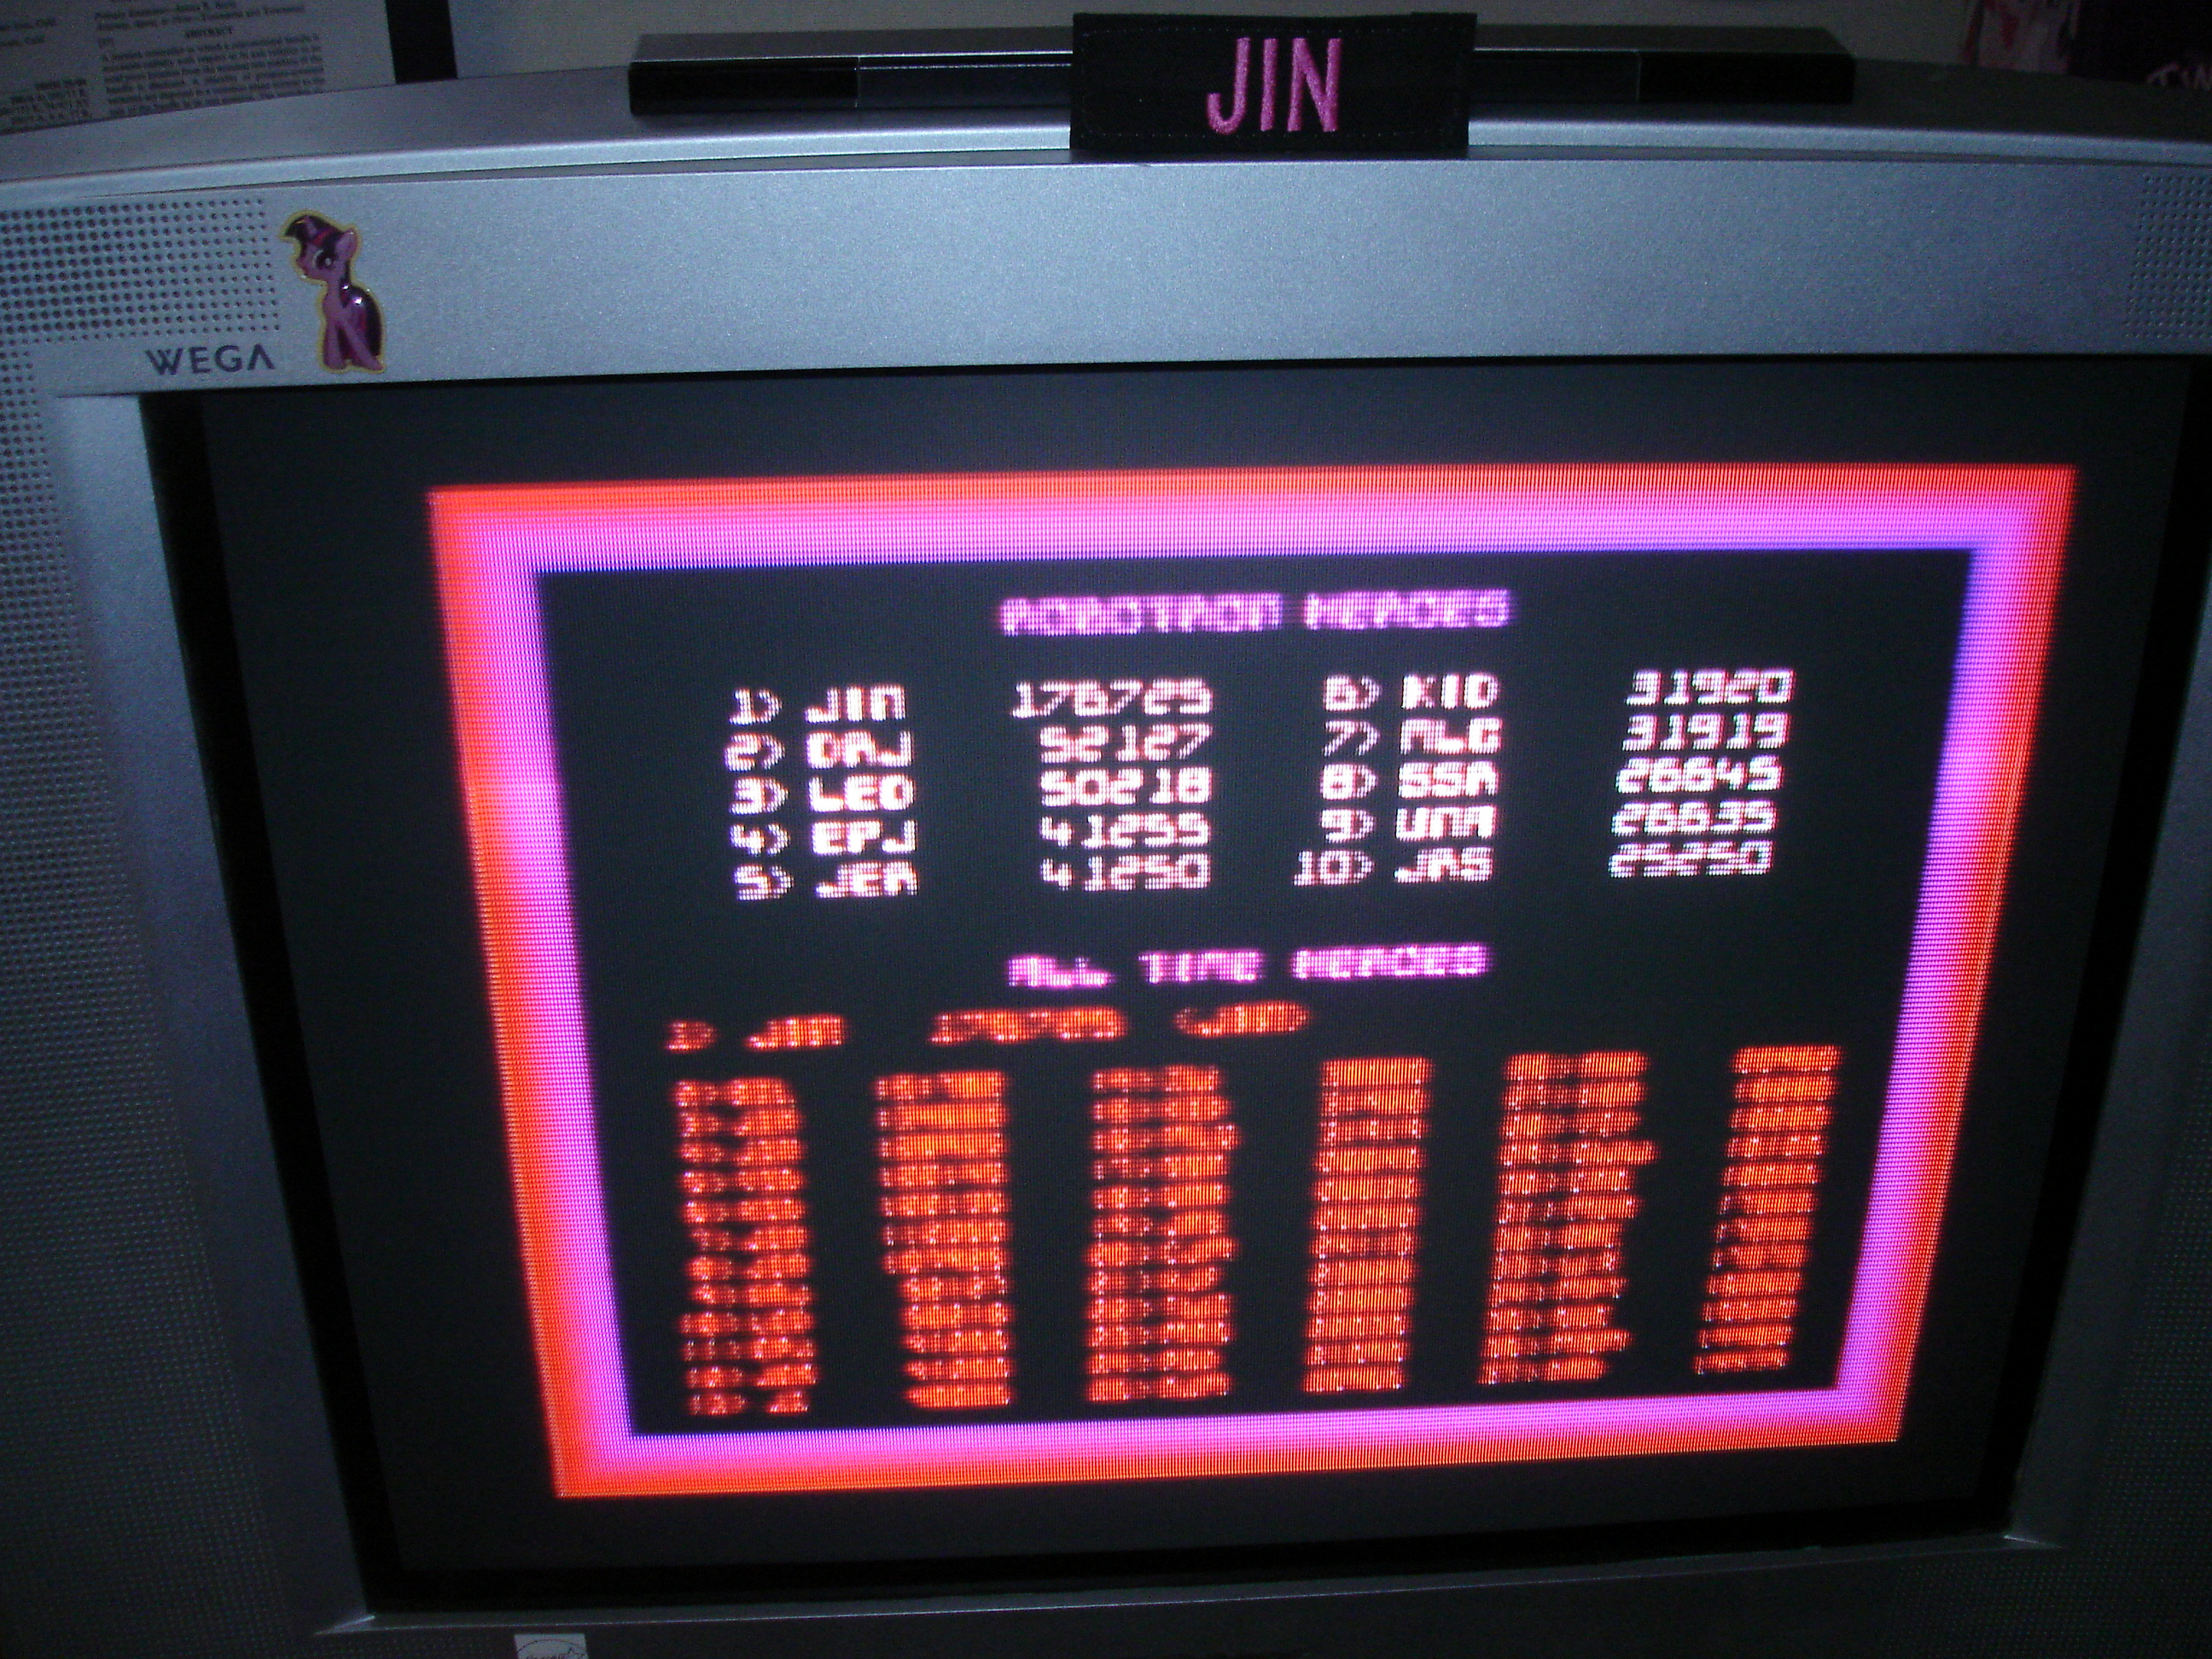
\includegraphics[width=0.8\linewidth]{Figures/web1.jpg}
  \centering
  \caption{Original high score board}
  \label{fig:web1}
\end{figure}


\begin{figure}[H]
  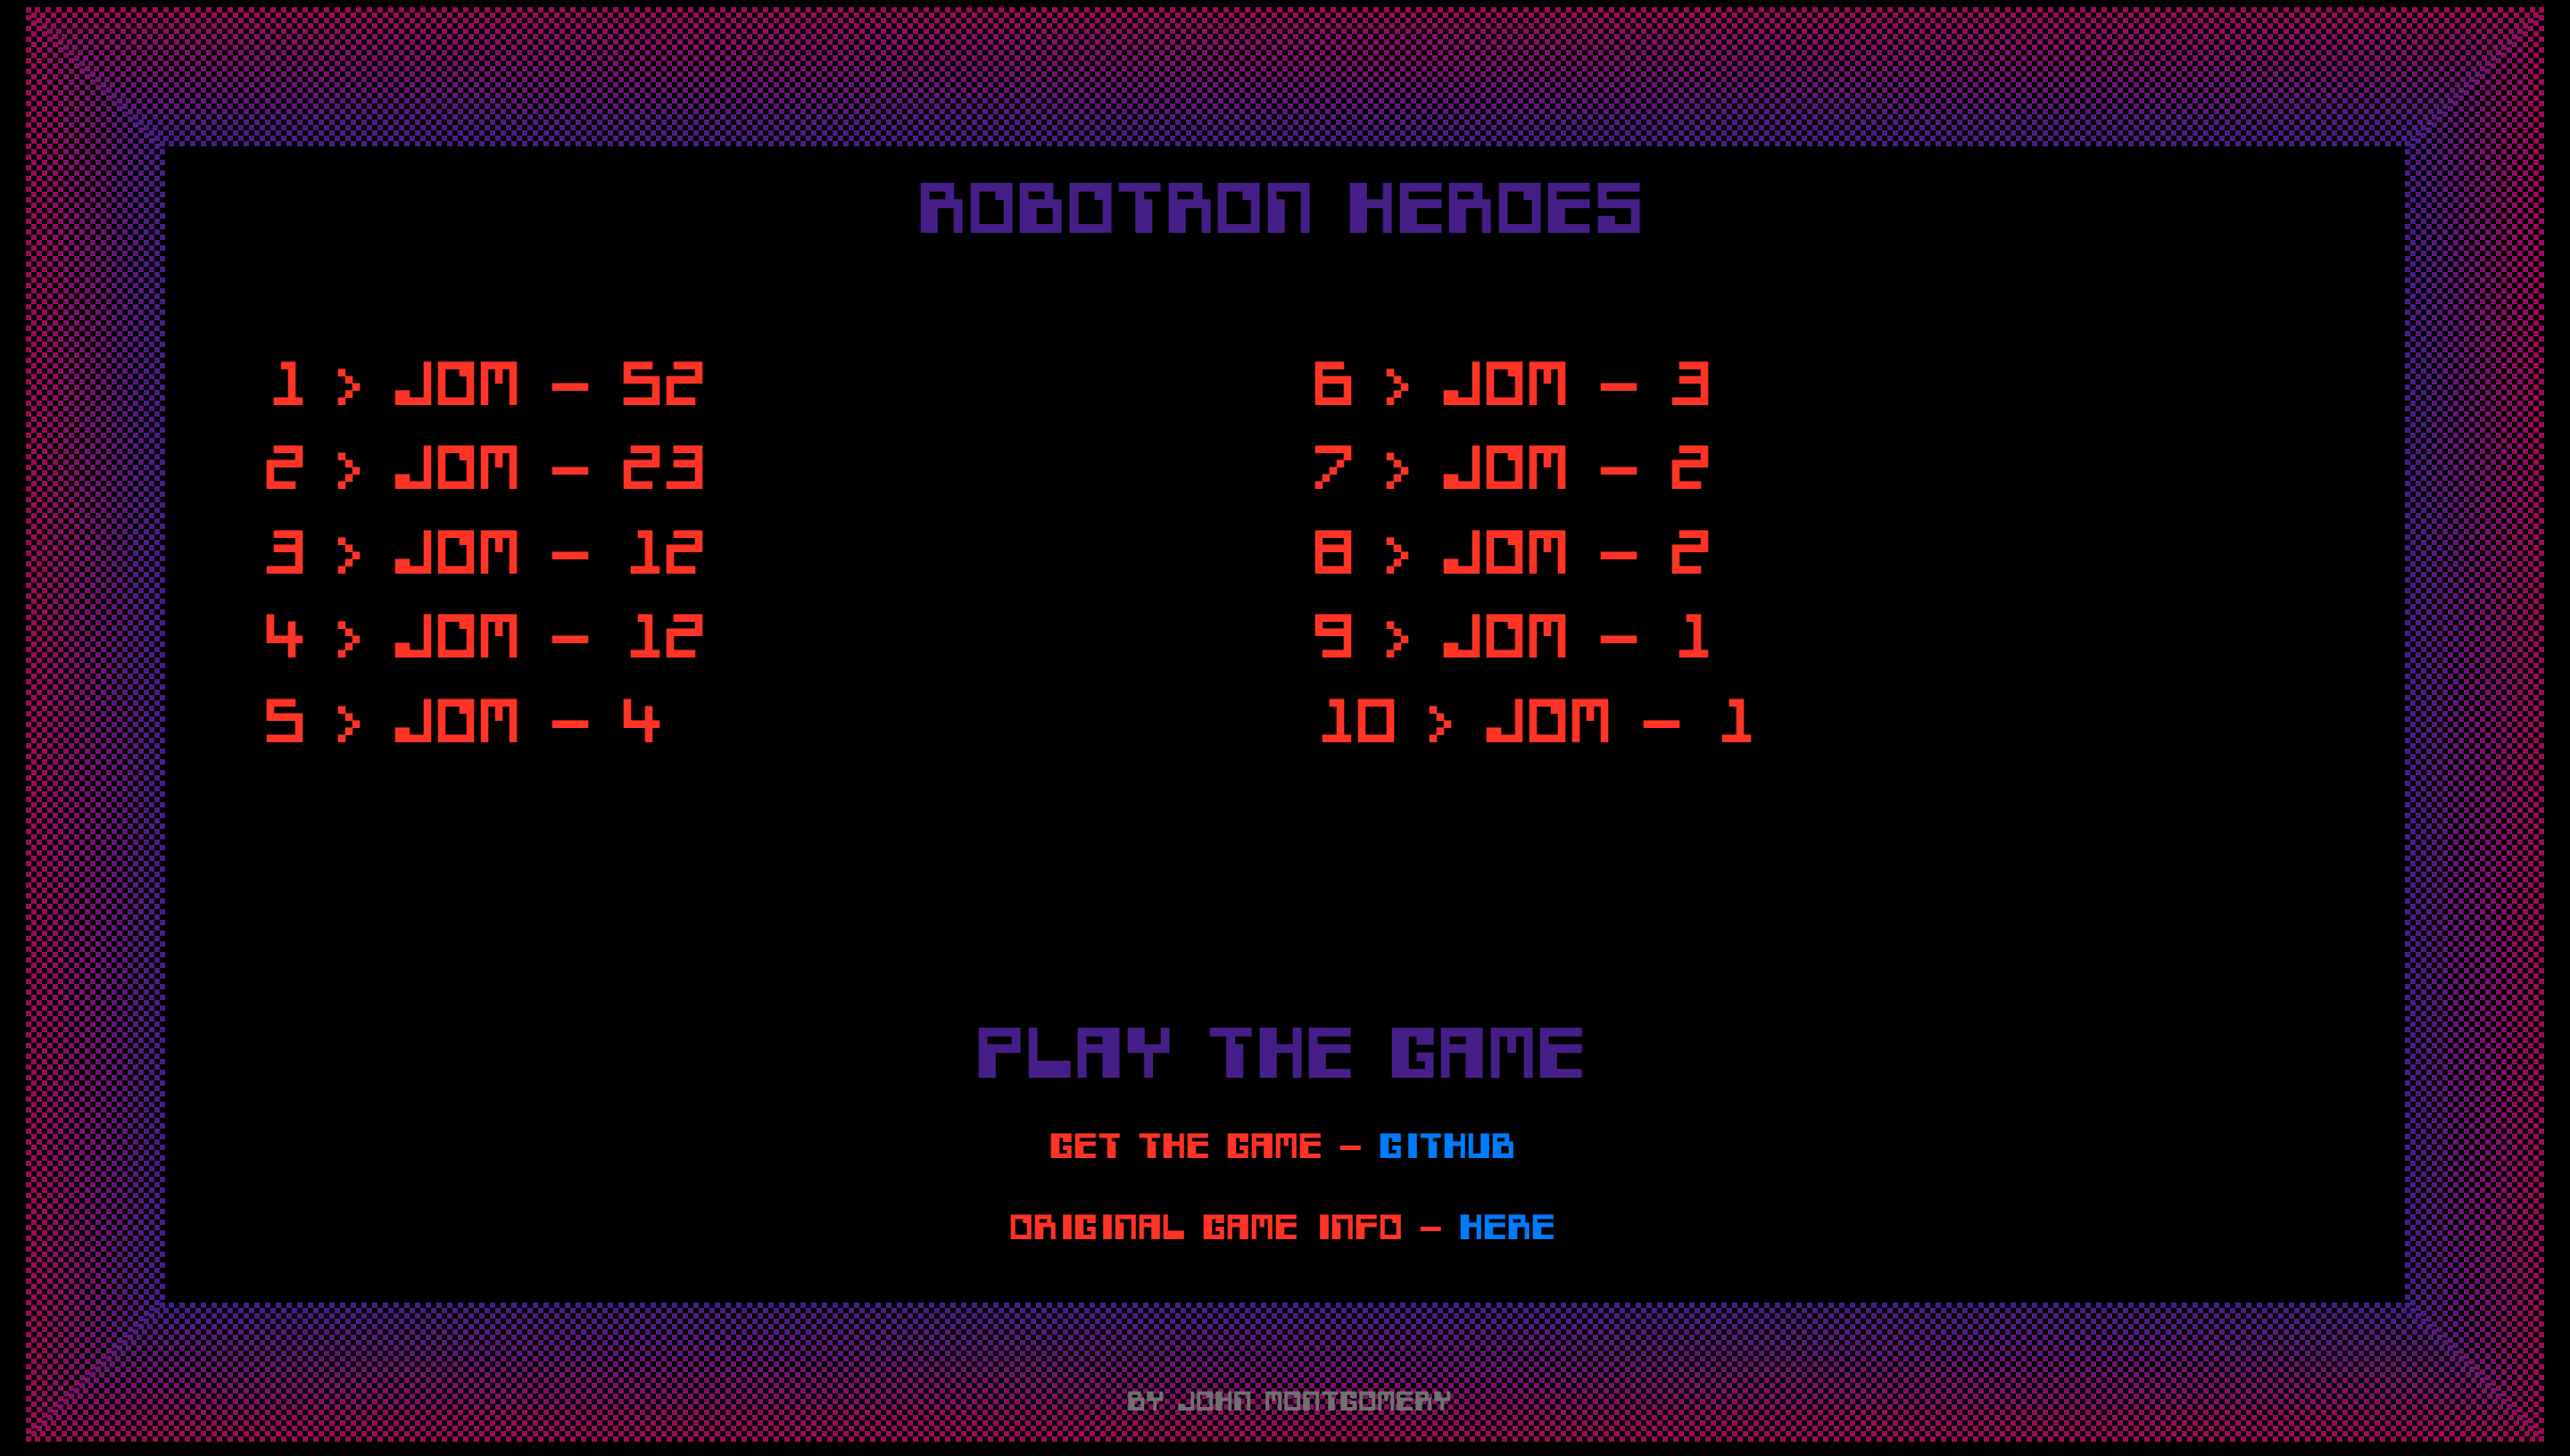
\includegraphics[width=0.8\linewidth]{Figures/web2.png}
  \centering
  \caption{My web implementation of the site}
  \label{fig:web2}
\end{figure}

\section{Database Design}
The database will be needed for the back end of the website, and also is needed in order to make the API work - it stores all the information about the games played, allowing users to login from different clients, and keeps users logged in with tokens, even when they stop running the game. This set up doesn't necessarily need a very complex database set up, it i1s more than proficient with simply having 3 tables, one for main login info, one for scores and one for tokens. The  design puts it into the 3rd normal form to ensure the best time and space efficiency. The SQL statements were tested and written for a sqlite database.

\subsection{Tables (ERD's)}
This diagram shows the database design. It is quite simple, and consists of 2 one to many relationships. One user can have many scores, and one user can have many tokens. This is handled with the foreign key id which allows the tables to be linked, and efficiently get the needed values with join statements.

\begin{figure}[H]
  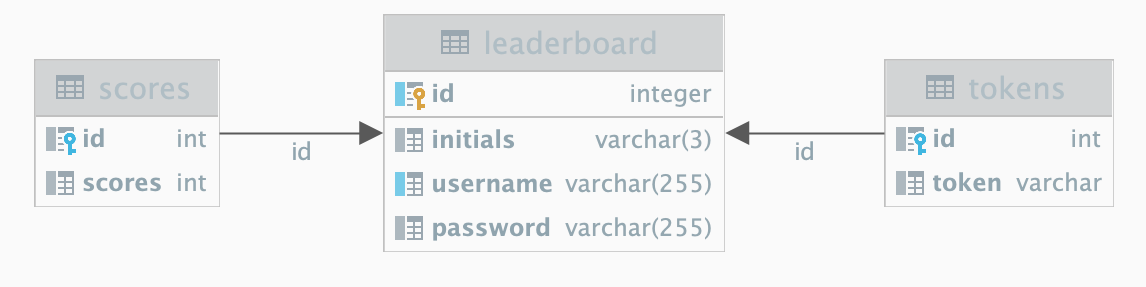
\includegraphics[width=0.8\linewidth]{Figures/leaderboard.png}
  \centering
  \caption{ERD showing the database design}
  \label{fig:ERD}
\end{figure}

\subsection{Queries}
This section will detail all the queries used in the code, in order of how they are found in the file, it just so happens this is also essentially in order of the complexity. The first query is run every time the flask server is run. By using 'IF NOT EXISTS' i am able to ensure that the table will be there when needed, but also that restarting the server will not remove any data which is stored in the file. 

\begin{figure}[H]
    \begin{lstlisting}[language=SQL, style=mystyle1]
CREATE TABLE IF NOT EXISTS leaderboard (
    id INTEGER UNIQUE PRIMARY KEY AUTOINCREMENT,
    initials VARCHAR(3),
    username VARCHAR(255) UNIQUE,
    password VARCHAR(255)
);
CREATE TABLE IF NOT EXISTS scores(
    id INT references leaderboard,
    scores INT
);
CREATE TABLE IF NOT EXISTS tokens (
    id INT references leaderboard,
    token VARCHAR
);
    \end{lstlisting}
      \centering
      \caption{Create table queries}
      \label{fig:SQL1}
\end{figure}

This select is used to return the top 10 scorers in the database, deconstructing it, we can see we are selecting the initials and scores, from the leader board table, joined to the scores table, on the id's. Next we want to order by the scores to ensure we get the top 10, and then only select 10 items
\begin{figure}[H]
    \begin{lstlisting}[language=SQL, style=mystyle1]
SELECT leaderboard.initials, scores
FROM leaderboard
LEFT JOIN scores
ON leaderboard.id = scores.id
ORDER BY scores DESC
LIMIT 10;
    \end{lstlisting}
      \centering
      \caption{Query to get the top 10 scorers and the initals linked to them}
      \label{fig:SQL2}
\end{figure}


\begin{figure}[H]
    \begin{lstlisting}[language=SQL, style=mystyle1]
SELECT leaderboard.id
FROM leaderboard
WHERE leaderboard.username = {username}
LIMIT 1;
    \end{lstlisting}
      \centering
      \caption{Query to get the id of a user given their unique username}
      \label{fig:SQL3}
\end{figure}

\begin{figure}[H]
    \begin{lstlisting}[language=SQL, style=mystyle1]
SELECT password
FROM leaderboard
WHERE leaderboard.id = {userid}
LIMIT 1;
    \end{lstlisting}
      \centering
      \caption{Query to get the hashed password info for a given id}
      \label{fig:SQL4}
\end{figure}

\begin{figure}[H]
    \begin{lstlisting}[language=SQL, style=mystyle1]
SELECT token
FROM tokens
WHERE id = {userid}
LIMIT 1;
    \end{lstlisting}
      \centering
      \caption{Query to get the token for a given id}
      \label{fig:SQL5}
\end{figure}

\begin{figure}[H]
    \begin{lstlisting}[language=SQL, style=mystyle1]
INSERT INTO tokens (id, token)
VALUES ('{userid}','{token}');
    \end{lstlisting}
      \centering
      \caption{Query to insert the token values}
      \label{fig:SQL6}
\end{figure}

\begin{figure}[H]
    \begin{lstlisting}[language=SQL, style=mystyle1]
INSERT INTO scores (id, scores)
VALUES ({userid},{score});
    \end{lstlisting}
      \centering
      \caption{Query to insert a new score}
      \label{fig:SQL7}
\end{figure}

\begin{figure}[H]
    \begin{lstlisting}[language=SQL, style=mystyle1]
INSERT INTO leaderboard (initials, username, password)
VALUES ('{initials}','{username}','{tostore}');
    \end{lstlisting}
      \centering
      \caption{Query to insert a new score}
      \label{fig:SQL8}
\end{figure}



\section{HCI}
Human Computer Interaction designs are going to be taken from the pygame itself, as this is how my program was built. I will also show some screens from the original game, all of which are taken from the links which can be found in the analysis section. The font is found at \url{https://fontstruct.com/fontstructions/show/474939/robotron_2084} and is under a creative commons license.

\newpage
This screen we can see a bunch of random coloured squares, this is designed to look just like what startup did on the original arcade game of this. It has no real features to mention
\begin{figure}[H]
  \includegraphics[width=1\linewidth]{Figures/random.png}
  \centering
  \caption{Random screen shown}
  \label{fig:HCI1}
\end{figure}
\newpage
This testing screen (whilst probably useful for the original) is not functional, but gives a but more of the sense of the game. 
\begin{figure}[H]
  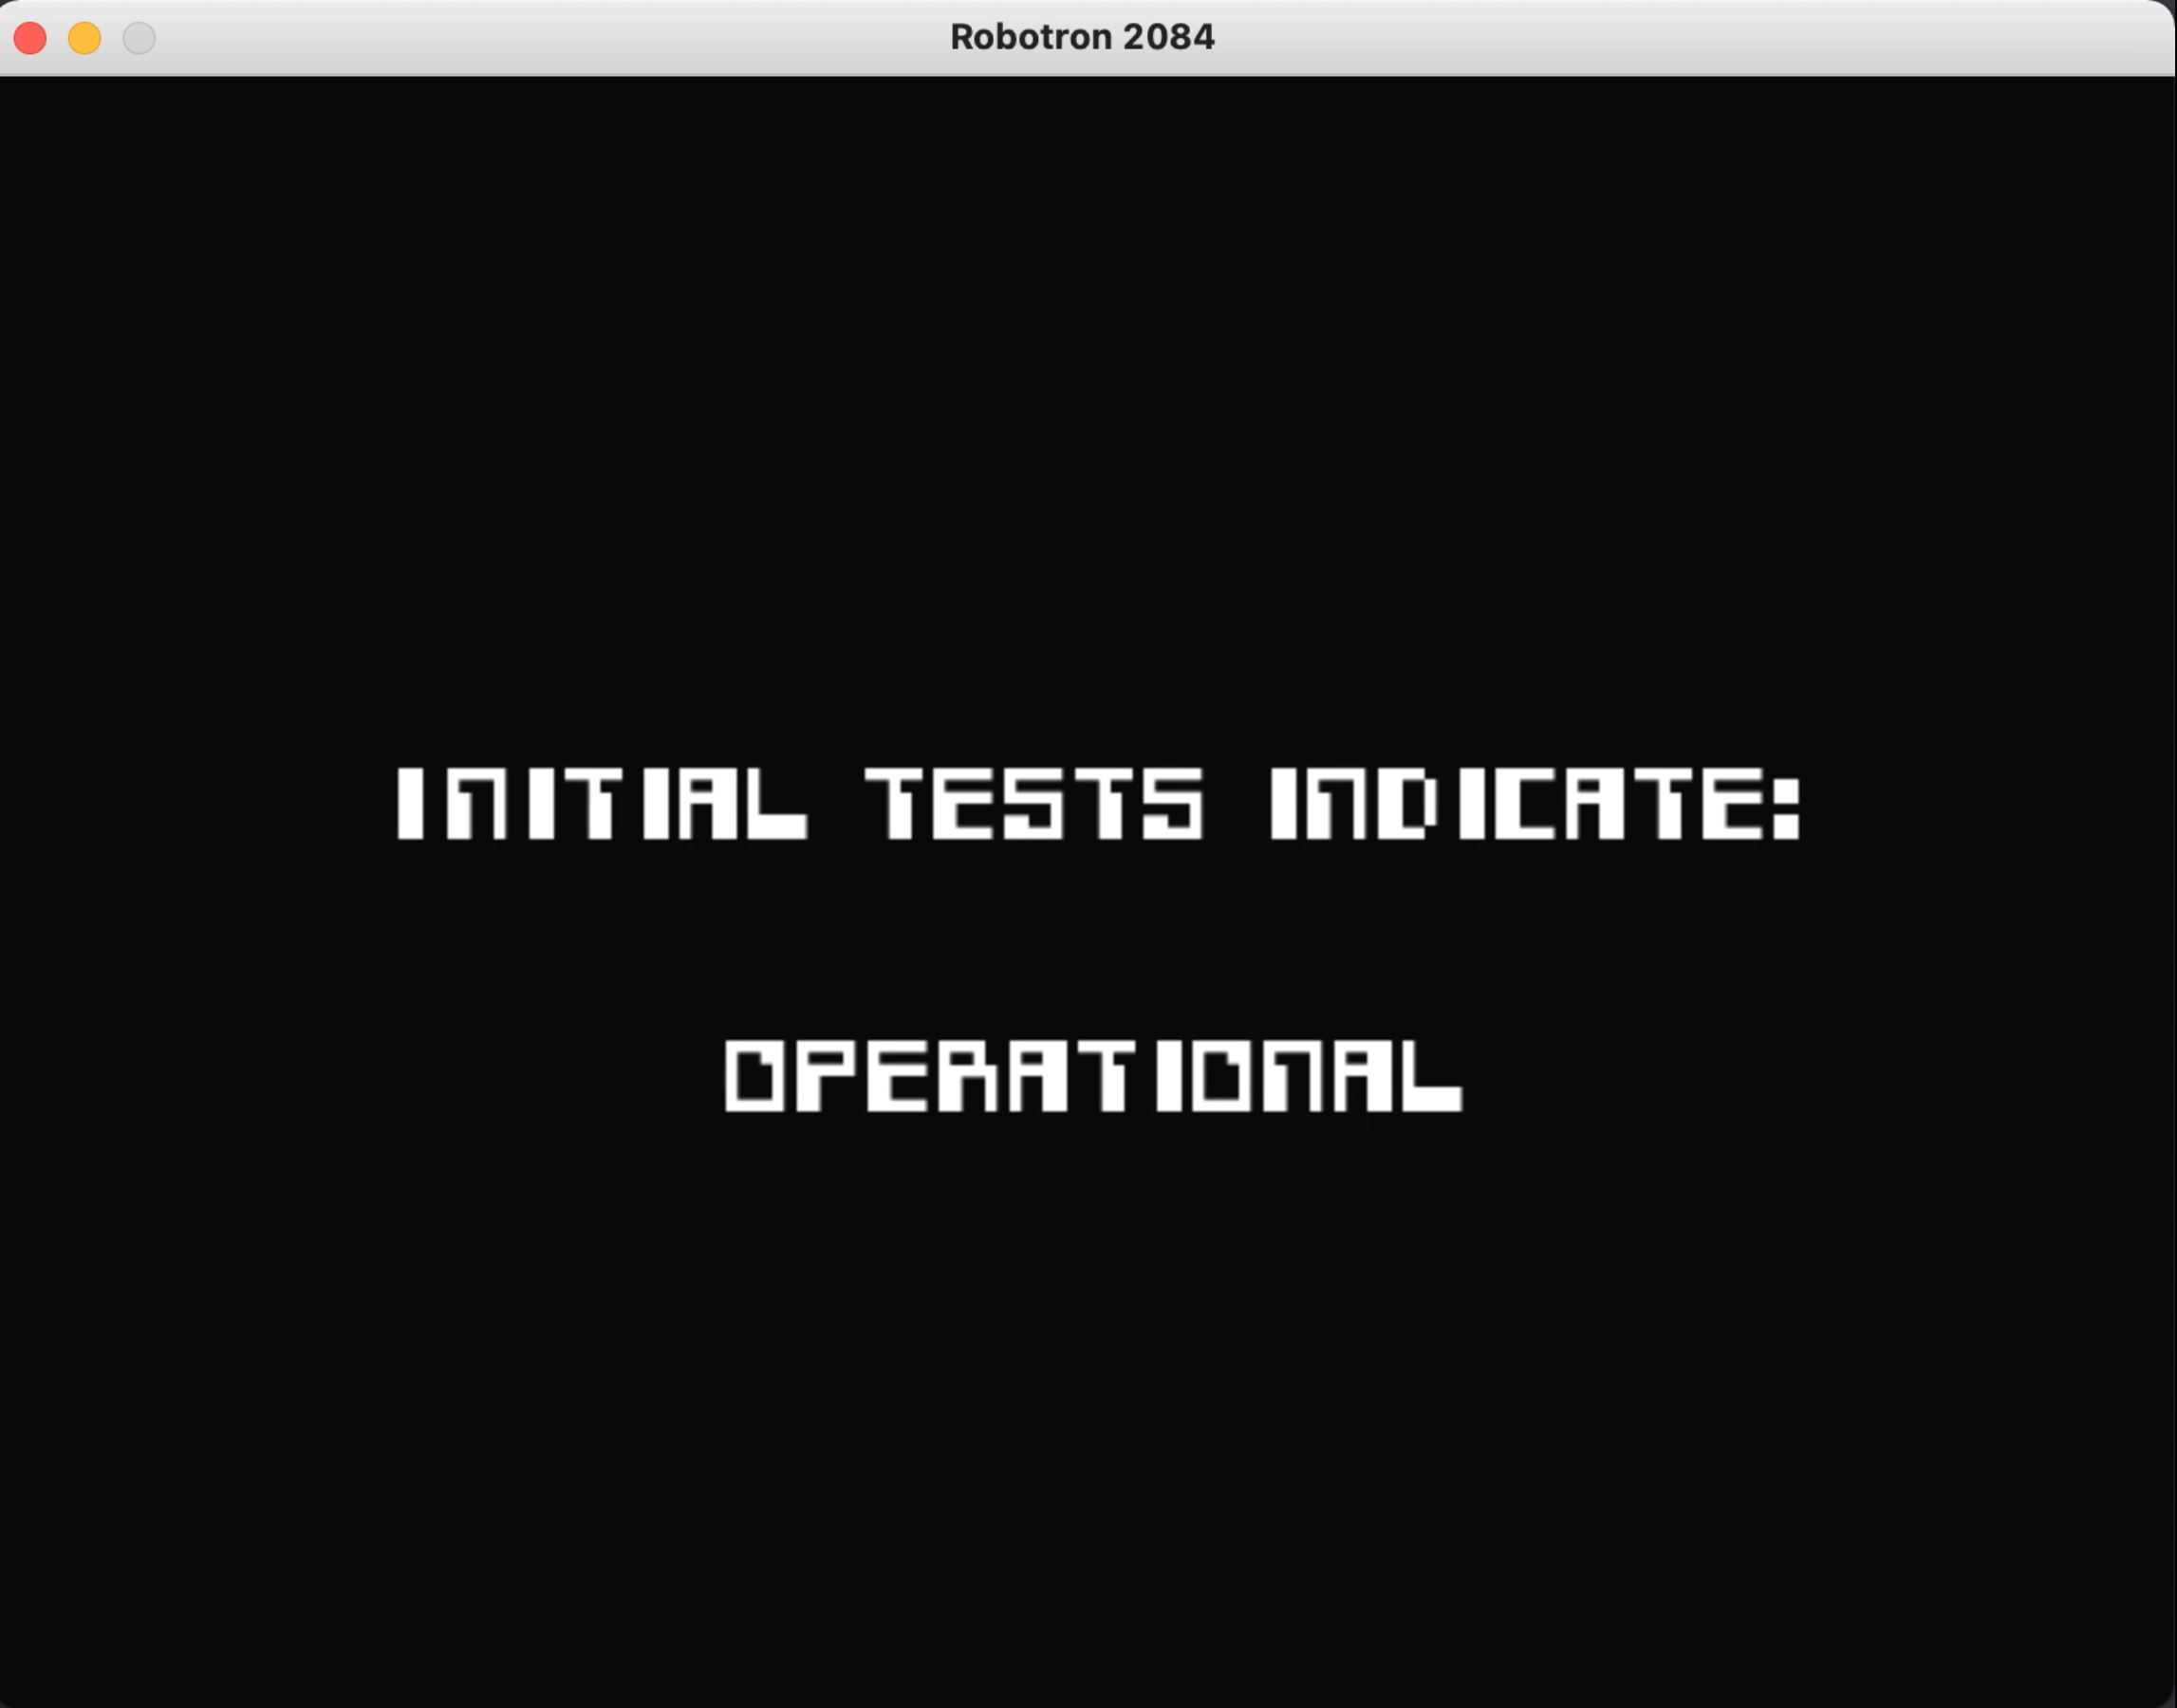
\includegraphics[width=1\linewidth]{Figures/tests.png}
  \centering
  \caption{Testing screen}
  \label{fig:HCI2}
\end{figure}

\newpage
This is the first part where users can actually interact, and it is a first into into the very fast pace of the game, with all the flashing colours and other rapidly changing features. This is where users can log in, play and get info like the leaderboard link.
\begin{figure}[H]
  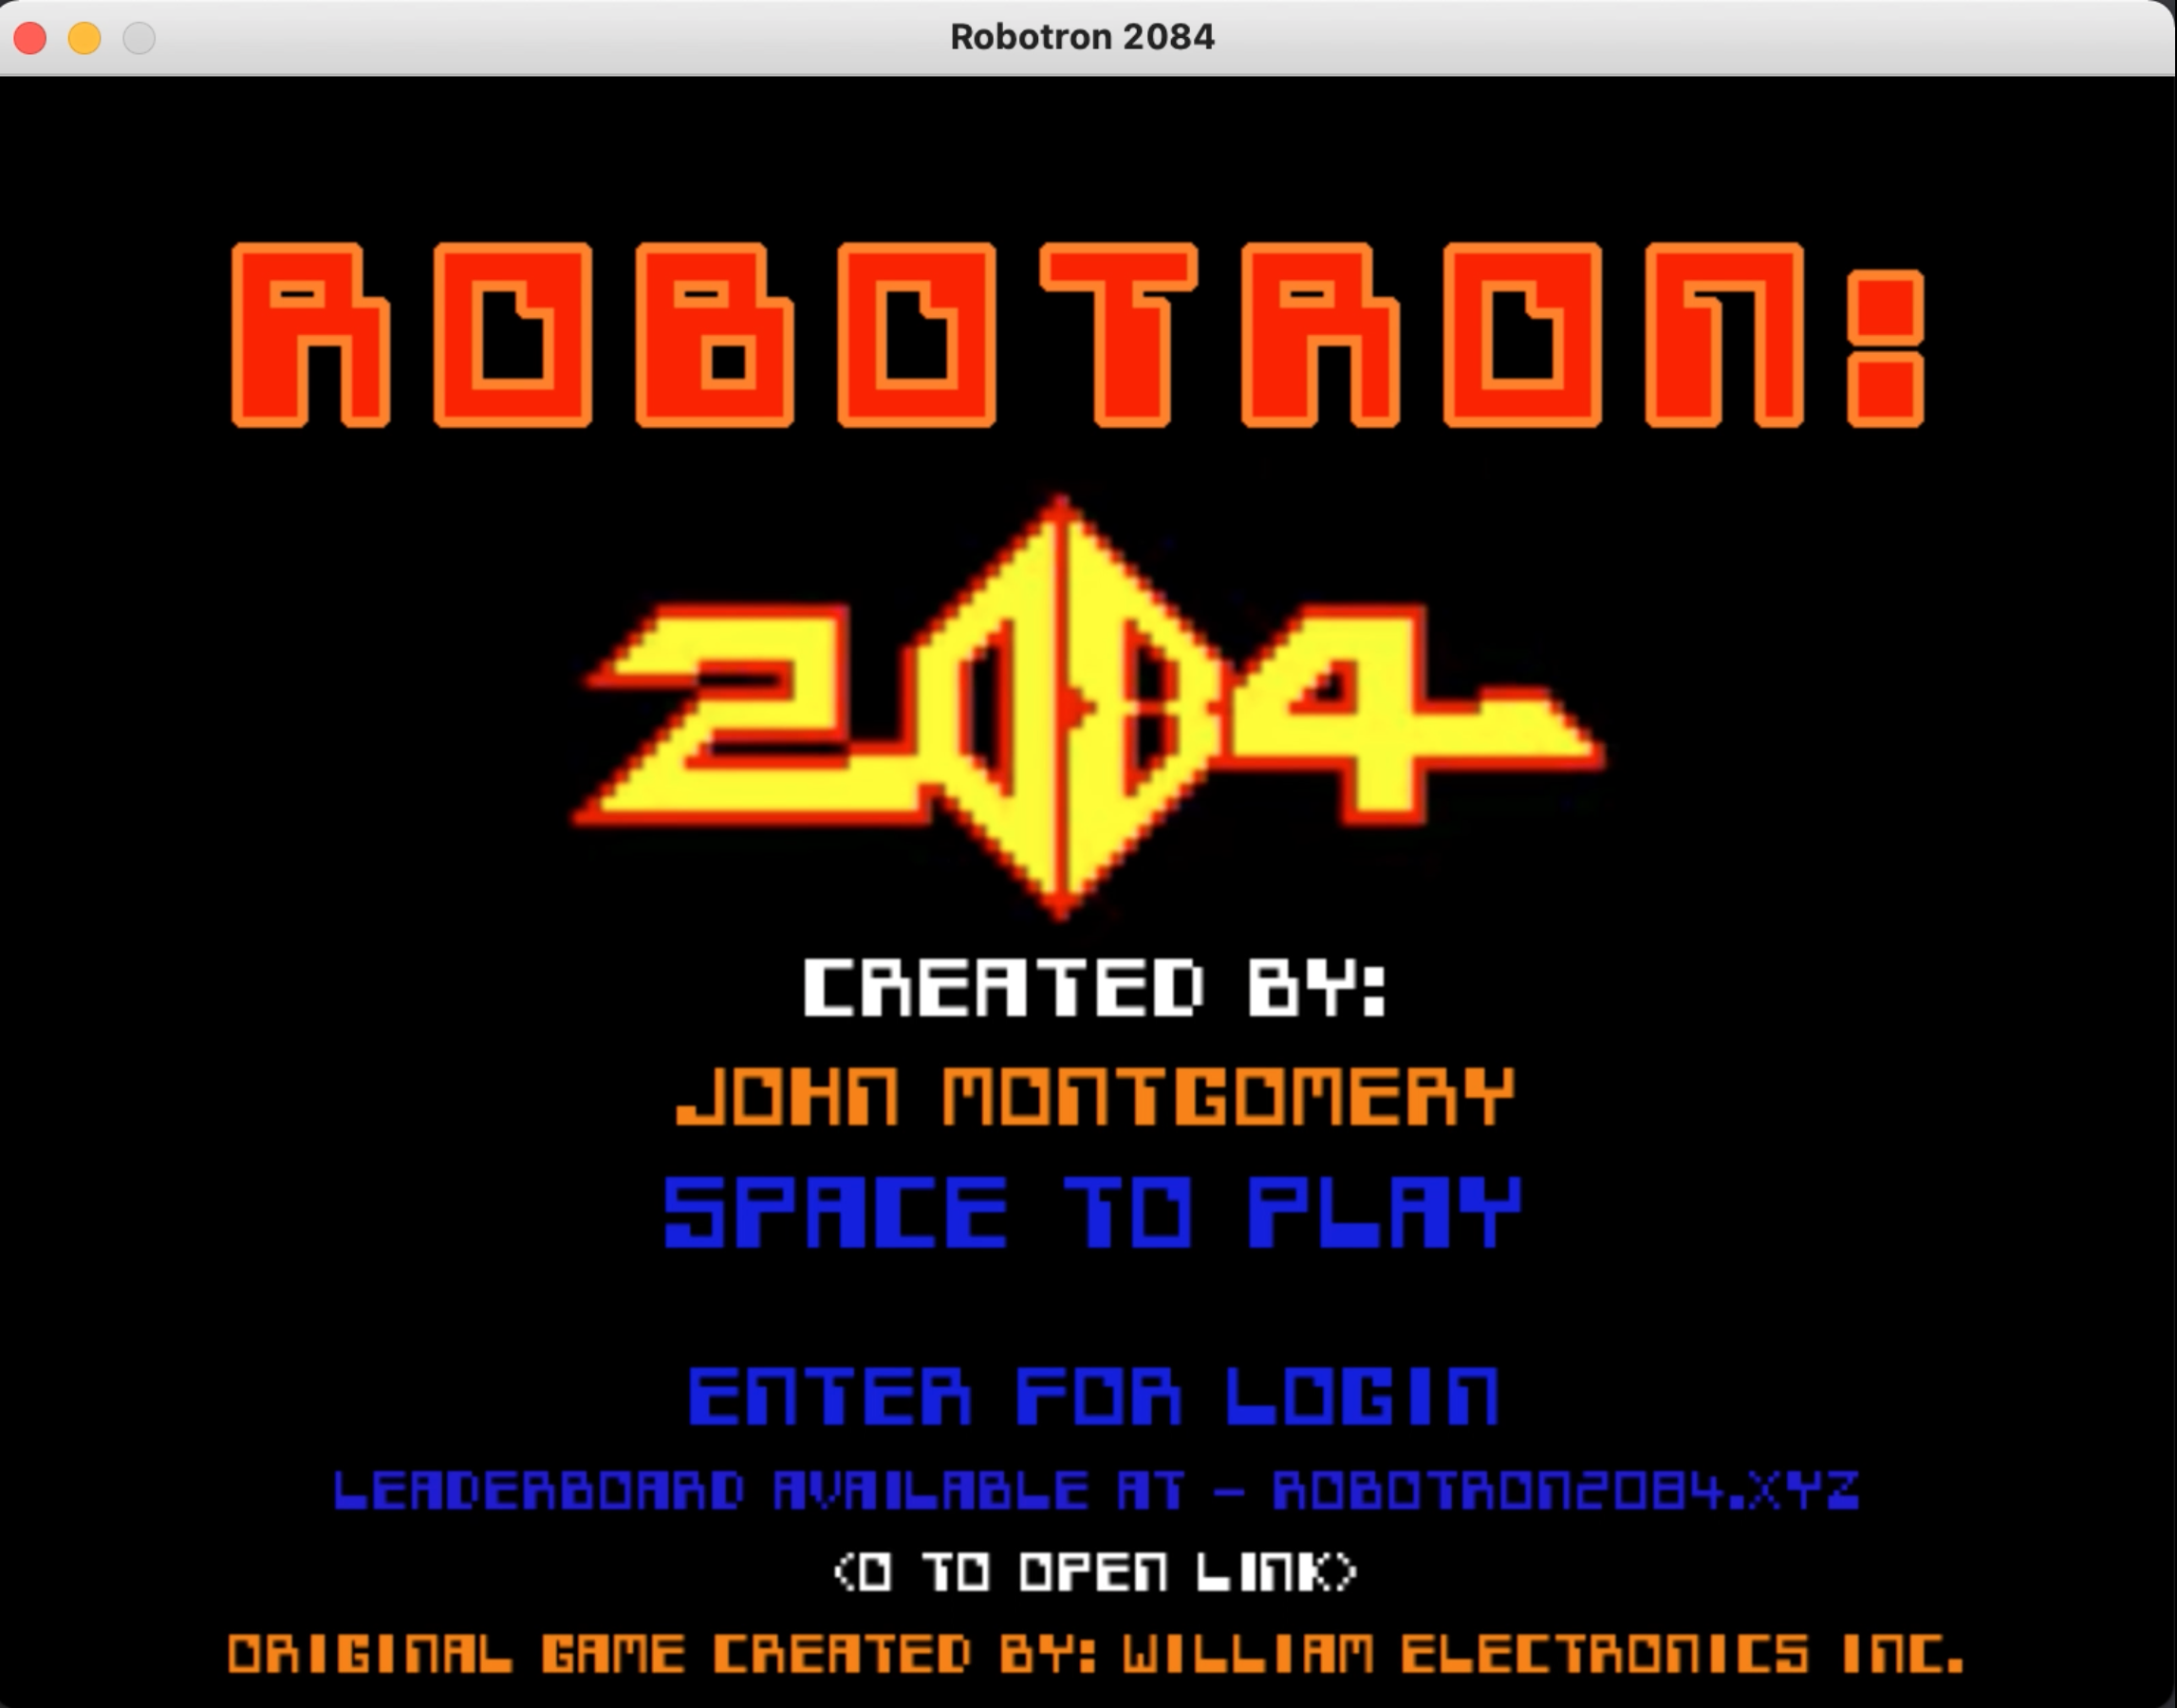
\includegraphics[width=1\linewidth]{Figures/menu.png}
  \centering
  \caption{Menu}
  \label{fig:HCI3}
\end{figure}
\newpage
This page is where the user logs in, it needs to be fairly basic, and it doesnt have all the flashing colours and brightness. The boxes get 'highlighted' when clicked, and there is a back button in the top left. The boxes also get bordered in red when the inputs are invalid, whether from an incorrect password or from other issues, like too short passwords.
\begin{figure}[H]
  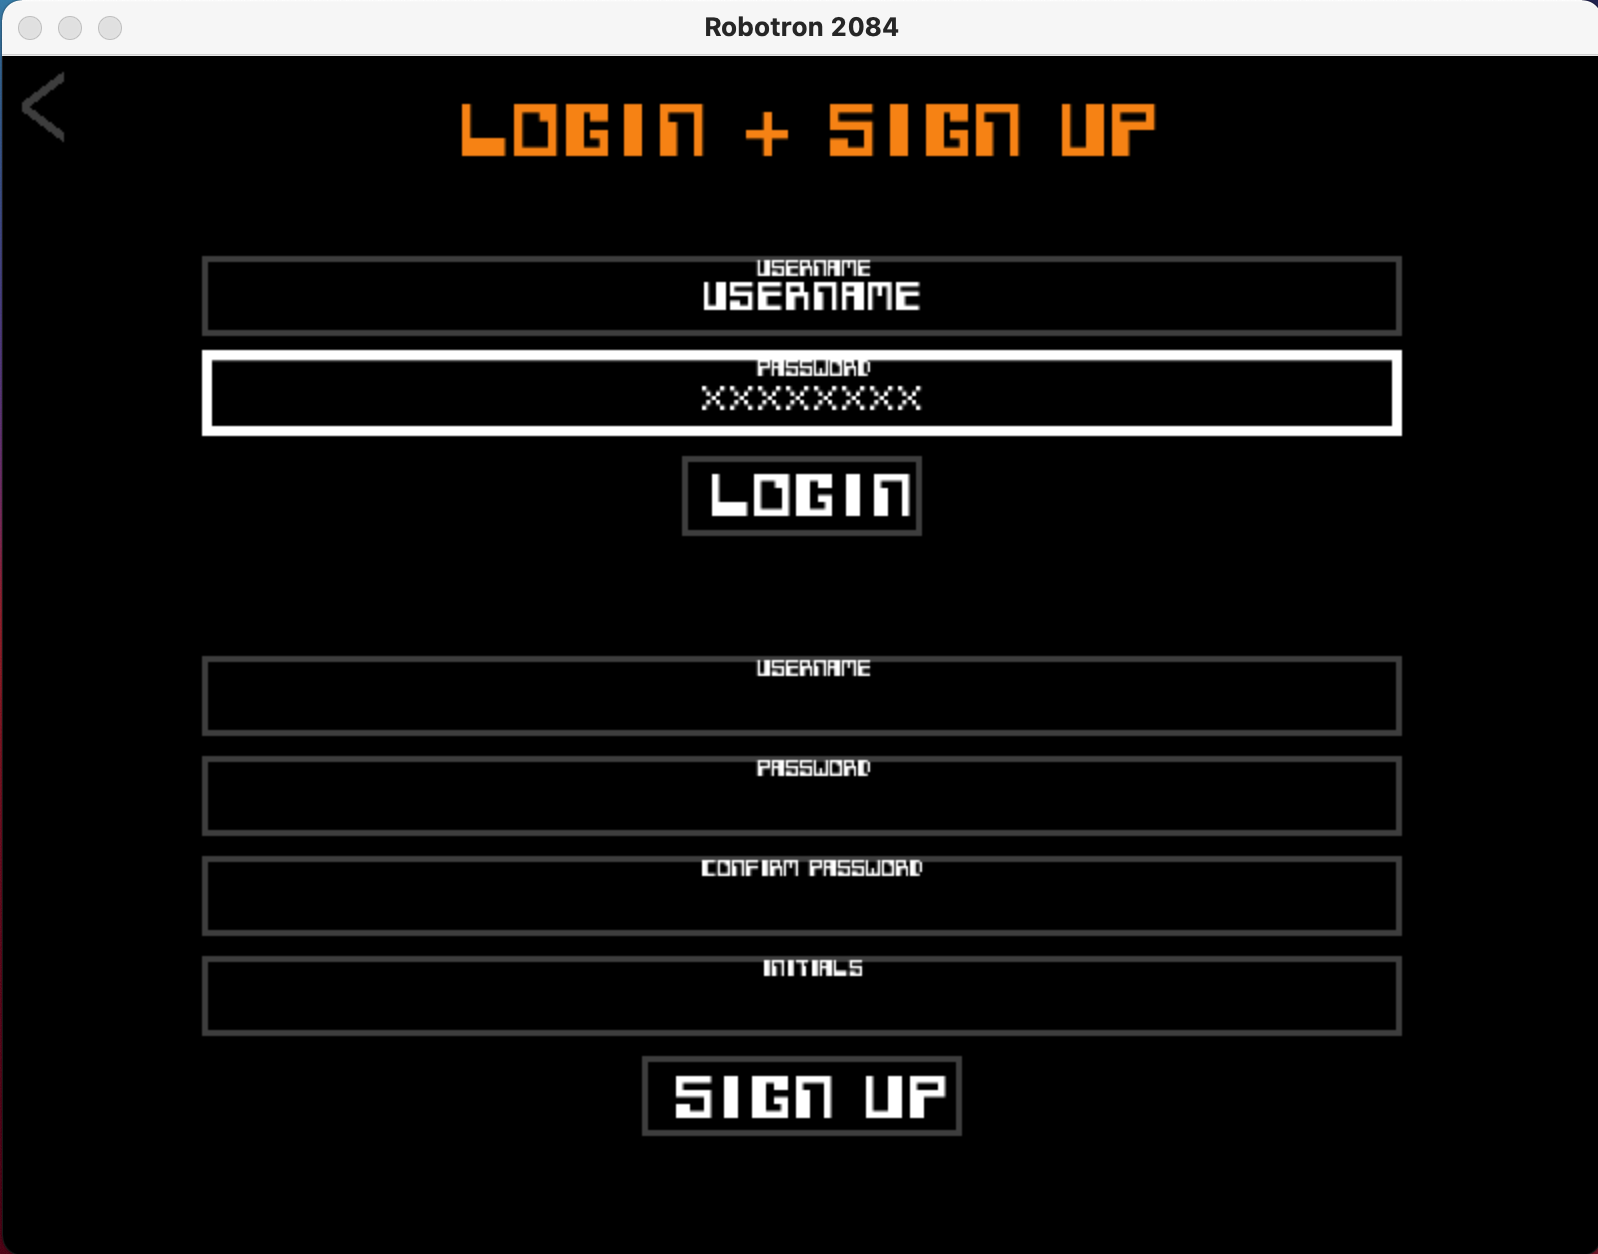
\includegraphics[width=1\linewidth]{Figures/login.png}
  \centering
  \caption{Login and sign up page}
  \label{fig:HCI4}
\end{figure}
\newpage
Theres not much variation from the original for this. Its very quick, and looks a lot like the basic game, bullets are random colours, and the border flashes, along with the life counter.
\begin{figure}[H]
  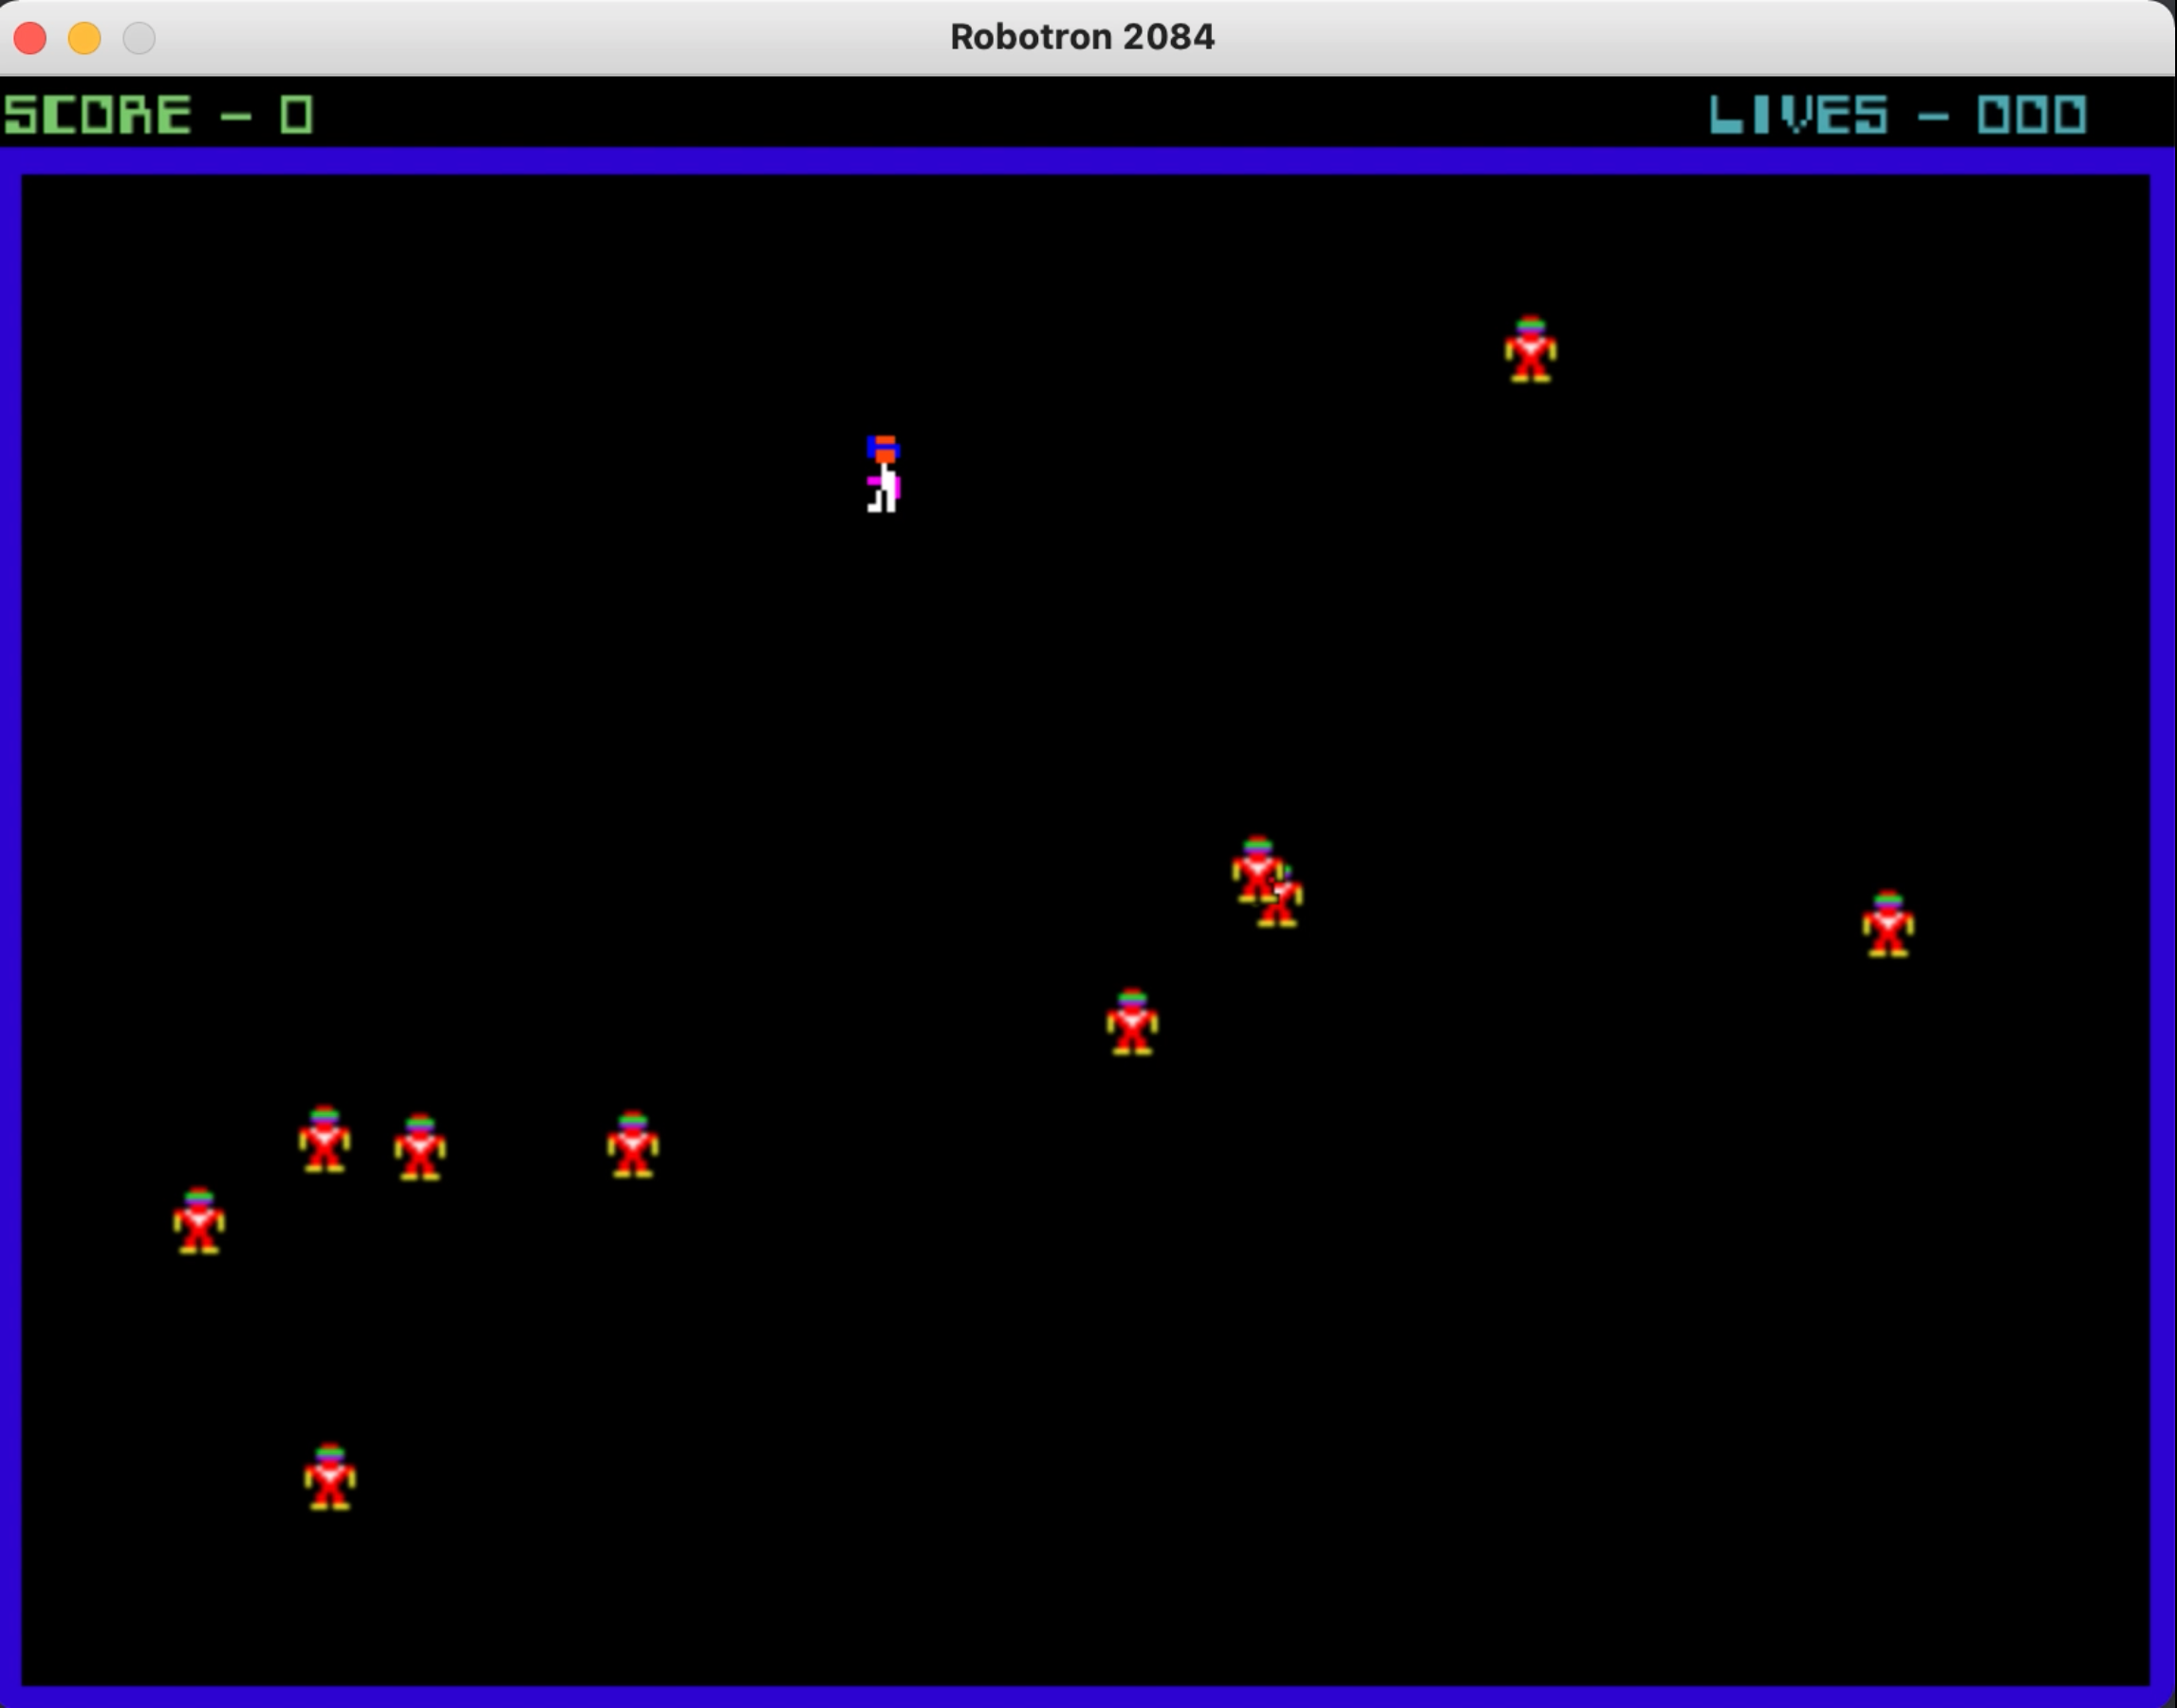
\includegraphics[width=1\linewidth]{Figures/gameplay.png}
  \centering
  \caption{Gameplay}
  \label{fig:HCI5}
\end{figure}
\newpage
This is as close as I could get to the original game, which uses a bit of a different design for the transition between levels.
\begin{figure}[H]
  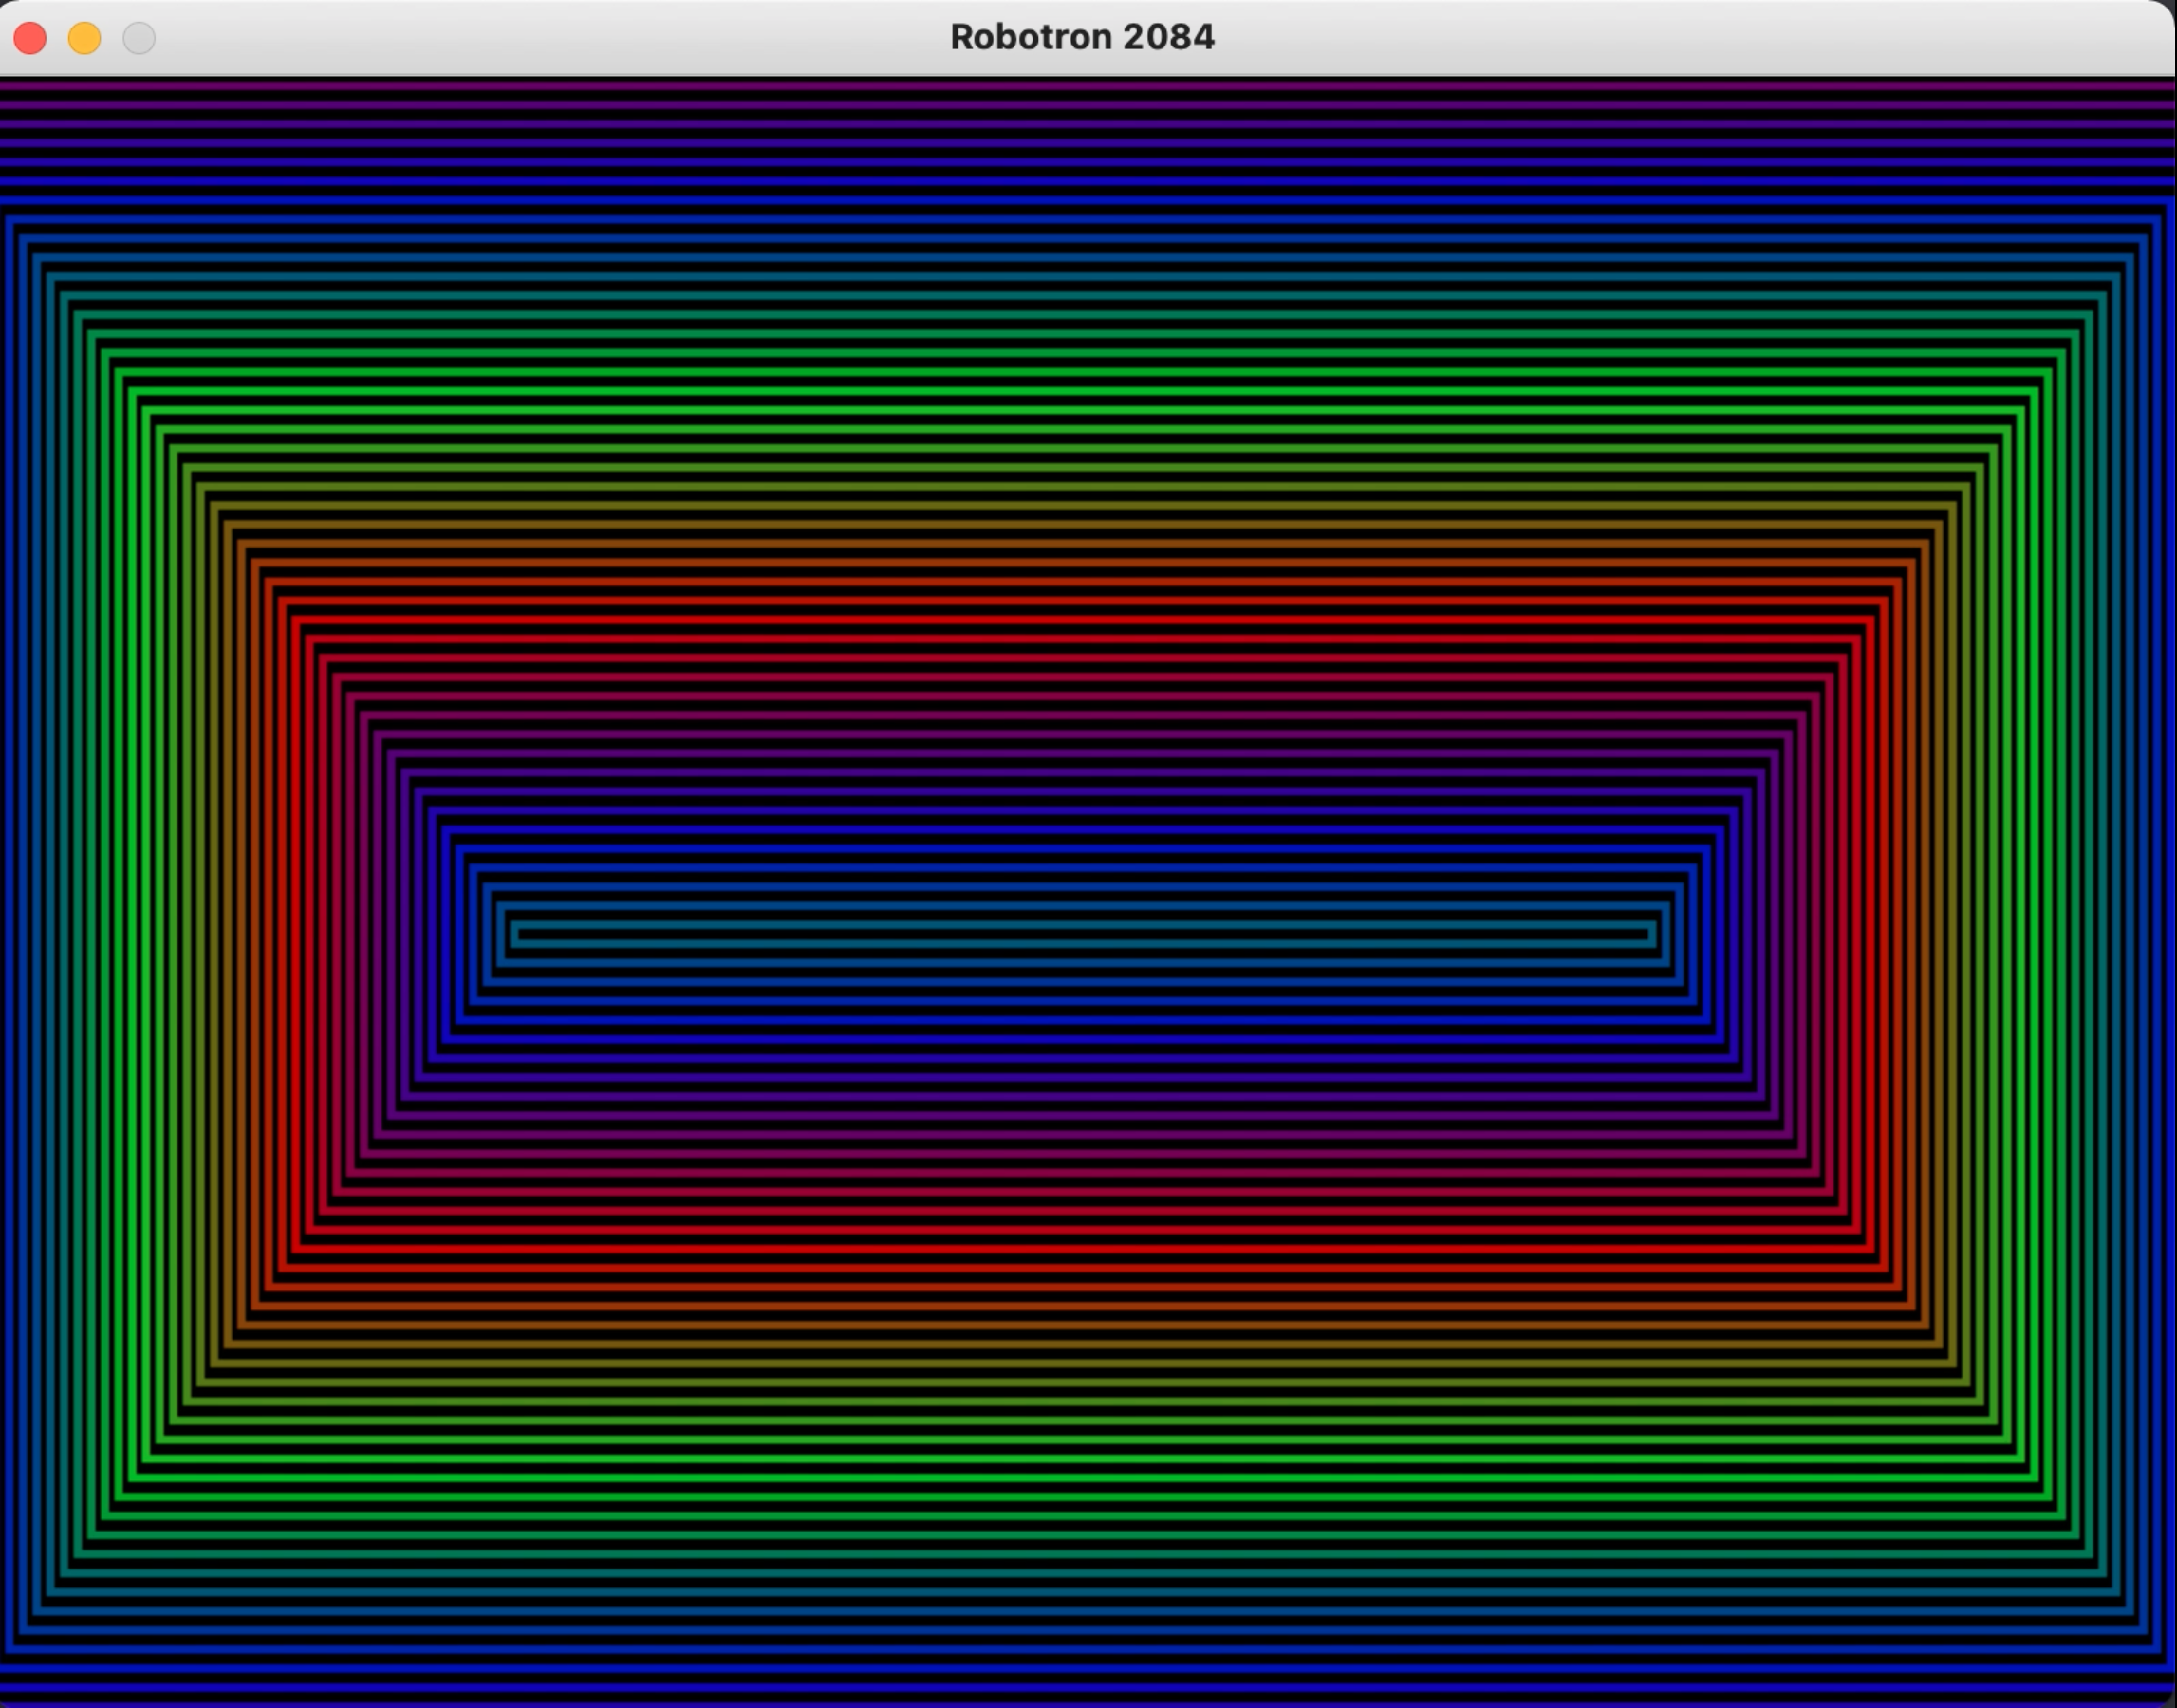
\includegraphics[width=1\linewidth]{Figures/trans.png}
  \centering
  \caption{Transition screen}
  \label{fig:HCI6}
\end{figure}